\section{ Evaluation}
\label{sec:Evaluation}

For the evaluation of \sysname, we are interested in two main aspects. First, we analyze the deduplication
performance of \sysname happening in the D-cluster~(\S\ref{sec:eval-dedup}). We then look at, how
the different B modes affect the performance of the primary cluster~(\S\ref{sec:eval-primary}).

%Our two-tier heterogeneous cache in the registry can improve the performance of the entire system
%by hiding the long latency imposed by the backend dedup system.
%Next, we present the preliminary evaluation of our user access history-based cache algorithm
%and the space efficiency of file cache.

%We conduct a performance evaluation of \sysname, and compare it with the modern registry setup~\cite{dockerworkload}.
%We start with describing the testbed and workloads then follow that with the evaluation results.
\subsection{Evaluation Setup}

Our testbed consists of 
%two clusters: 
%8-node client cluster and
%8-node registry cluster (Hulks), and
a 15-node cluster and
%Each client server is equipped with 32 cores, 64 GB RAM, 500 GB SSD, and 10,000Mb/s NIC. 
%Each client server is equipped with 8 cores, 64 GB RAM, 1 TB HDD, and 1000Mb/s NIC.
%During evaluation,
each node is equipped with 8 cores, 16\,GB RAM, a 500\,GB SSD, and a 10\,Gbps NIC. 
%We deploy Docker's registry container on each server and deploy a distributed Redis cluster on these 22 registry servers as our database.
%During our evaluation,
%we select different number of servers as our registry cluster
%and use the rest as client server.
%Note that each server only runs a single registry container
%while multiple clients can run on the same server.
%Besides,

%We instantiate multiple clients on each client server.
%backend registry storage cluster and frontend registry cache cluster. 
%Backend storage cluster includes 8 servers. 
%Each registry Hulk server is equipped with 32 cores, 64 GB RAM, 500 GB SSD, 1 TB HDD, and 10,000Mb/s NIC. 

%We implemented \sysname~cache on frontend cache cluster and installed \sysname~dedup on backend storage cluster. 
%We use extra 5 machines and each machine launches different number of clients to emulate client requests.
%Hulks and new hulks are used as backend.
%Thors are used as frontend.
%\subsection{}
\paragraph{Dataset}
%
%Recent work \cite{analysisdockergithub} conducts a comprehensive analysis of 47~TB Docker Hub images and reports that the popularity distribution of the images is heavily skewed.
%To evaluate how \sysname works for frequently accessed images, 
As our dataset, we download 74,000 popular images (i.e., images with a pull count greater than 100) from Docker Hub.
% 
The total size of this dataset is 12.5\,TB and contains 507,023 layers. 87.5\% of layers are smaller than 50\,MB.
%
After decompressing the layers, the total size of the dataset is 27.7\,TB.
%
Applying file-level deduplication on the decompressed dataset
reduces the total size of the dataset to only 7.2\,TB, yielding 
a deduplication ratio of 1.74.
%
%\Subil{is the dedup ratio $7.2\div27.7$ or $7.2\div12.5$? because neither of them equals 0.5. How is the dedup ratio calculated?}.
%
%The size distribution of our popular layer dataset is the same with the size distribution of~\cite{analysisdockergithub}.
%87.5\% of layers are smaller than 50 MB.
%12.3\% of layers fall between 50 MB and 1 GB.
%0.2\% of layers are bigger than 1 GB.
%Due to our testbed cluster's scaling restriction, 
%we set a limit to the layer size %\emph{layer size limitation} 
%at 250 MB. 
%Layers that are bigger than 250 MB are split into sub-layers.
%Based on our dataset analysis~\cite{xxx} and workload analysis~\cite{xxx},
%more than 90\% of layers are smaller than 50MB. 
%Therefore, we divided our sample dataset into two groups:
%smaller layers (layer size $\leq$ 50 MB) and big layers ( 50MB $\leq$ layer size $\leq$ 1 GB).
  
\paragraph{Workload}
%
To evaluate how \sysname performs for production registry workloads, 
we use the IBM Cloud Registry traces~\cite{dockerworkload}.
%
The traces come from three private registry clusters and 
four production registry clusters and span approximately 80 days.
%
As detailed in~\S\ref{sec:impl}, we randomly match layers from the four anonymized production
traces (\dal, \fra, \lon, and \syd) to layers from our dataset to generate four real-world production workloads.
%
Before an experiment, we first warmup P-servers and D-servers with a certain amount of layers as shown in
Table~\ref{tab:eval-overall} and then replay the first 5000 requests from each workload.
%
\Subil{there's nothing in the table indicating what number of layers we use for warmup.}
\LR{Do you mean we warm up the caches?}
%
Tables~\ref{tab:eval-overall} details how the 5000 requests for each workload are composed
with respect to layer and manifest requests.

%Note that we use a 3-way replication
%which triples the amount of data written during evaluation.
%We speedup trace replaying by using different speedup factors so that each trace finishes within 30 minutes.
%During all experiments,
%we set \emph{replication level} equal to 3.


\begin{table}[h!]
	%\centering
	%\tiny 
	\scriptsize
	\caption{Workload parameters.}
	\begin{tabular}{| c | c | c | c | c | c | c| c |} 
		\hline
	Trace    &   \#GET L & \#GET M & \#PUT L & \#PUT M & \#Uniq L & \#Uniq M \\ 
		\hline\hline
		Dal    &  2867  & 2000   & 124  & 9     & 1278 & 88      \\ 
		\hline
		Fra     &  1602  & 3278   & 111  & 9     & 420 & 43     \\
		\hline
		Lon    &  924    & 3972   & 98  & 6      & 698 & 88    \\
		\hline 
		Syd      &  1310   & 3653   & 35 & 2     & 154 & 18      \\  
		\hline
	\end{tabular}

\label{tab:eval-overall}
\end{table}


%\begin{table}[h!]
%	%\centering
%	\scriptsize 
%	\caption{Testing Dataset.}
%	\begin{tabular}{| c | c | c | c | c | } 
%		\hline
%		Trace  (GB)  &   Dataset  & Data transferred  & GET L size  & PUT L size  \\ 
%		\hline\hline
%		Dal   & 20  & 37 & 35 & 2    \\ 
%		\hline
%		Fra     & 6  & 16 & 14 & 2   \\
%		\hline
%		Lon    &10   &  14 &12  & 2      \\
%		\hline 
%		Syd      &  2  &  9 & 8 & 1      \\  
%		\hline
%	\end{tabular}
%	
%	\label{tab:eval-dataset}
%\end{table}


%\begin{figure}[t]
%	\centering
%	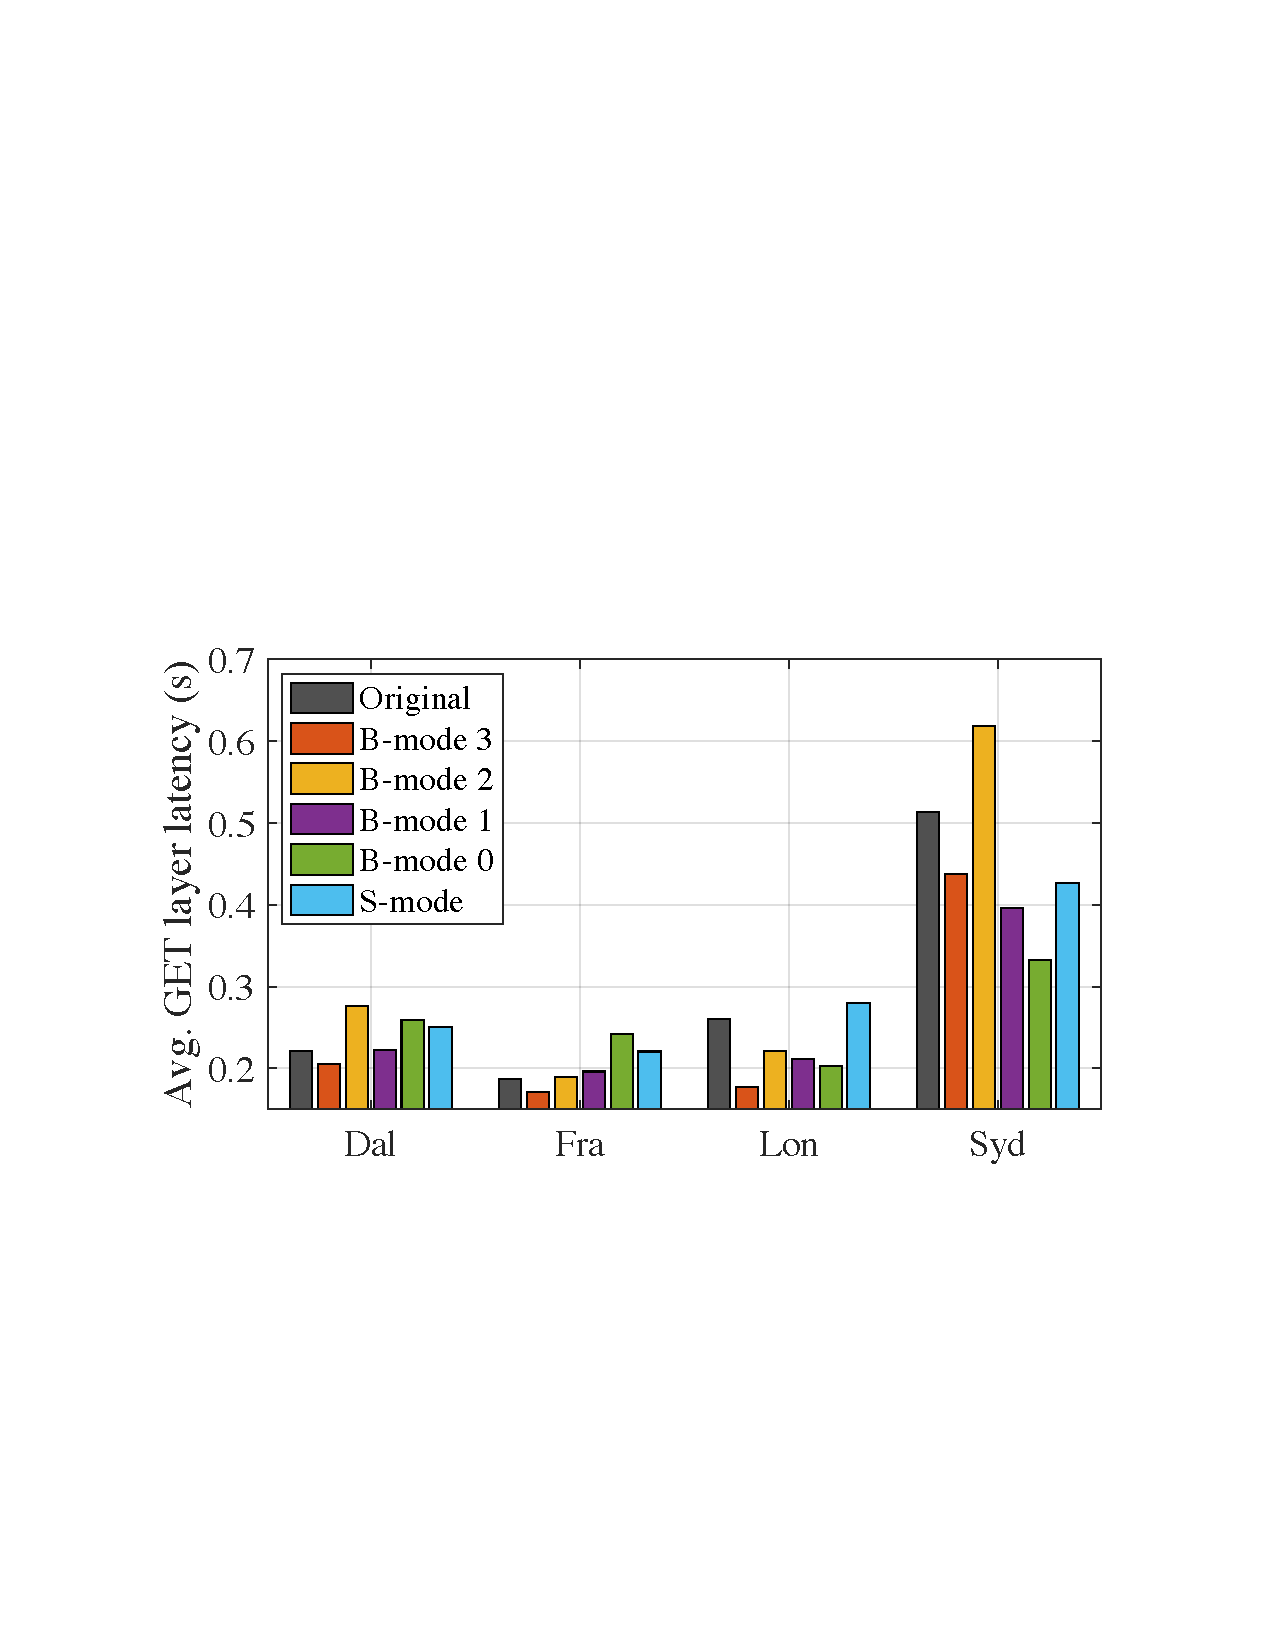
\includegraphics[width=0.45\textwidth]{graphs/get-layer-latency.pdf}
%	\caption{GET layer latency across different workloads from different schemes.}
%	%	\vspace{-3pt}
%	\label{fig:getlayerlatency}
%	
%\end{figure}



%In the following, we first present the performance comparison between original registry and \sysname.
%Next, we present the layer restoring performance.

\subsection{Deduplication Performance}
\label{sec:eval-dedup}

%We map the traces with two different layer groups: 
%small layers (layer size $\leq$ 50 MB)

\begin{figure*}[t]
	\centering
	\begin{minipage}{0.3\textwidth}
		\centering
		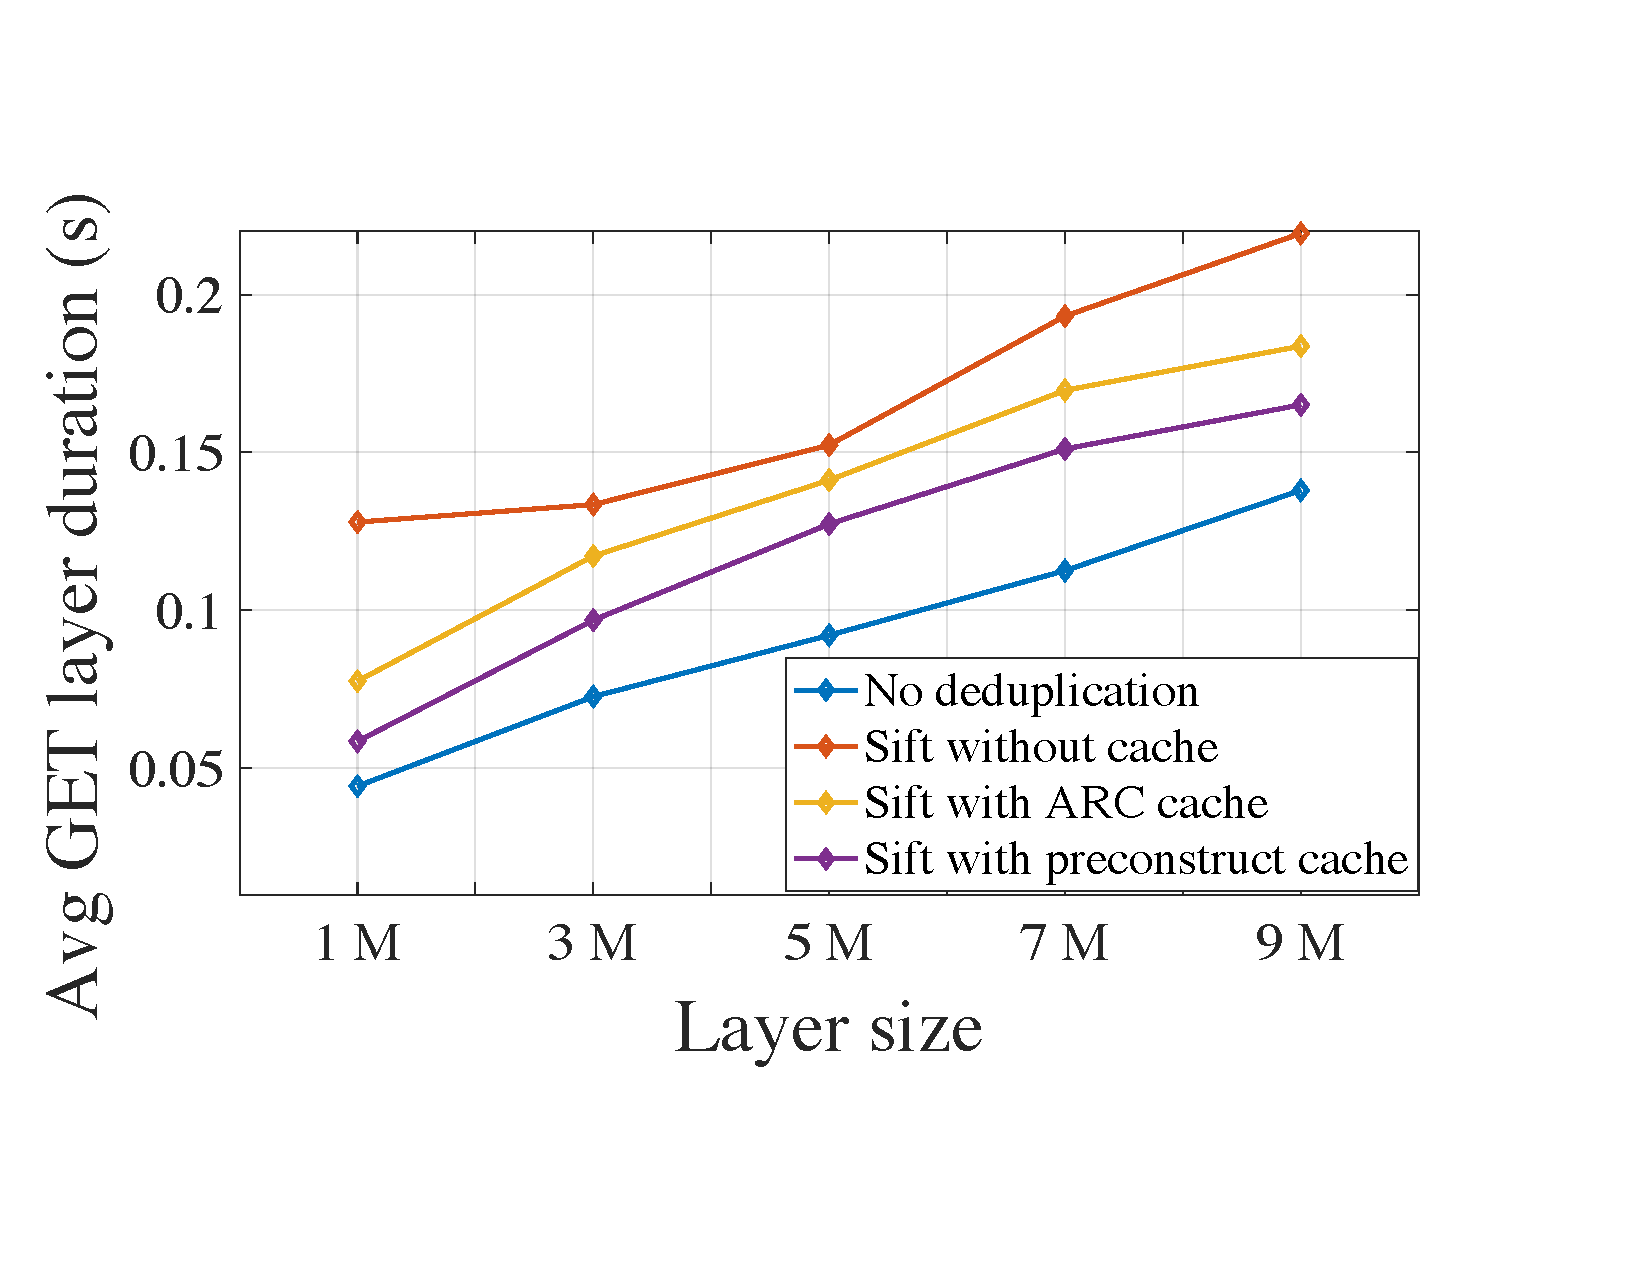
\includegraphics[width=\textwidth]{graphs/1nodegetlayerlatency.pdf}
		\caption{GET layer latency}
		\label{fig:eval-1nodegetlayerlatency}
	\end{minipage}%
\hspace{1mm}
	\begin{minipage}{0.29\textwidth}
		\centering
		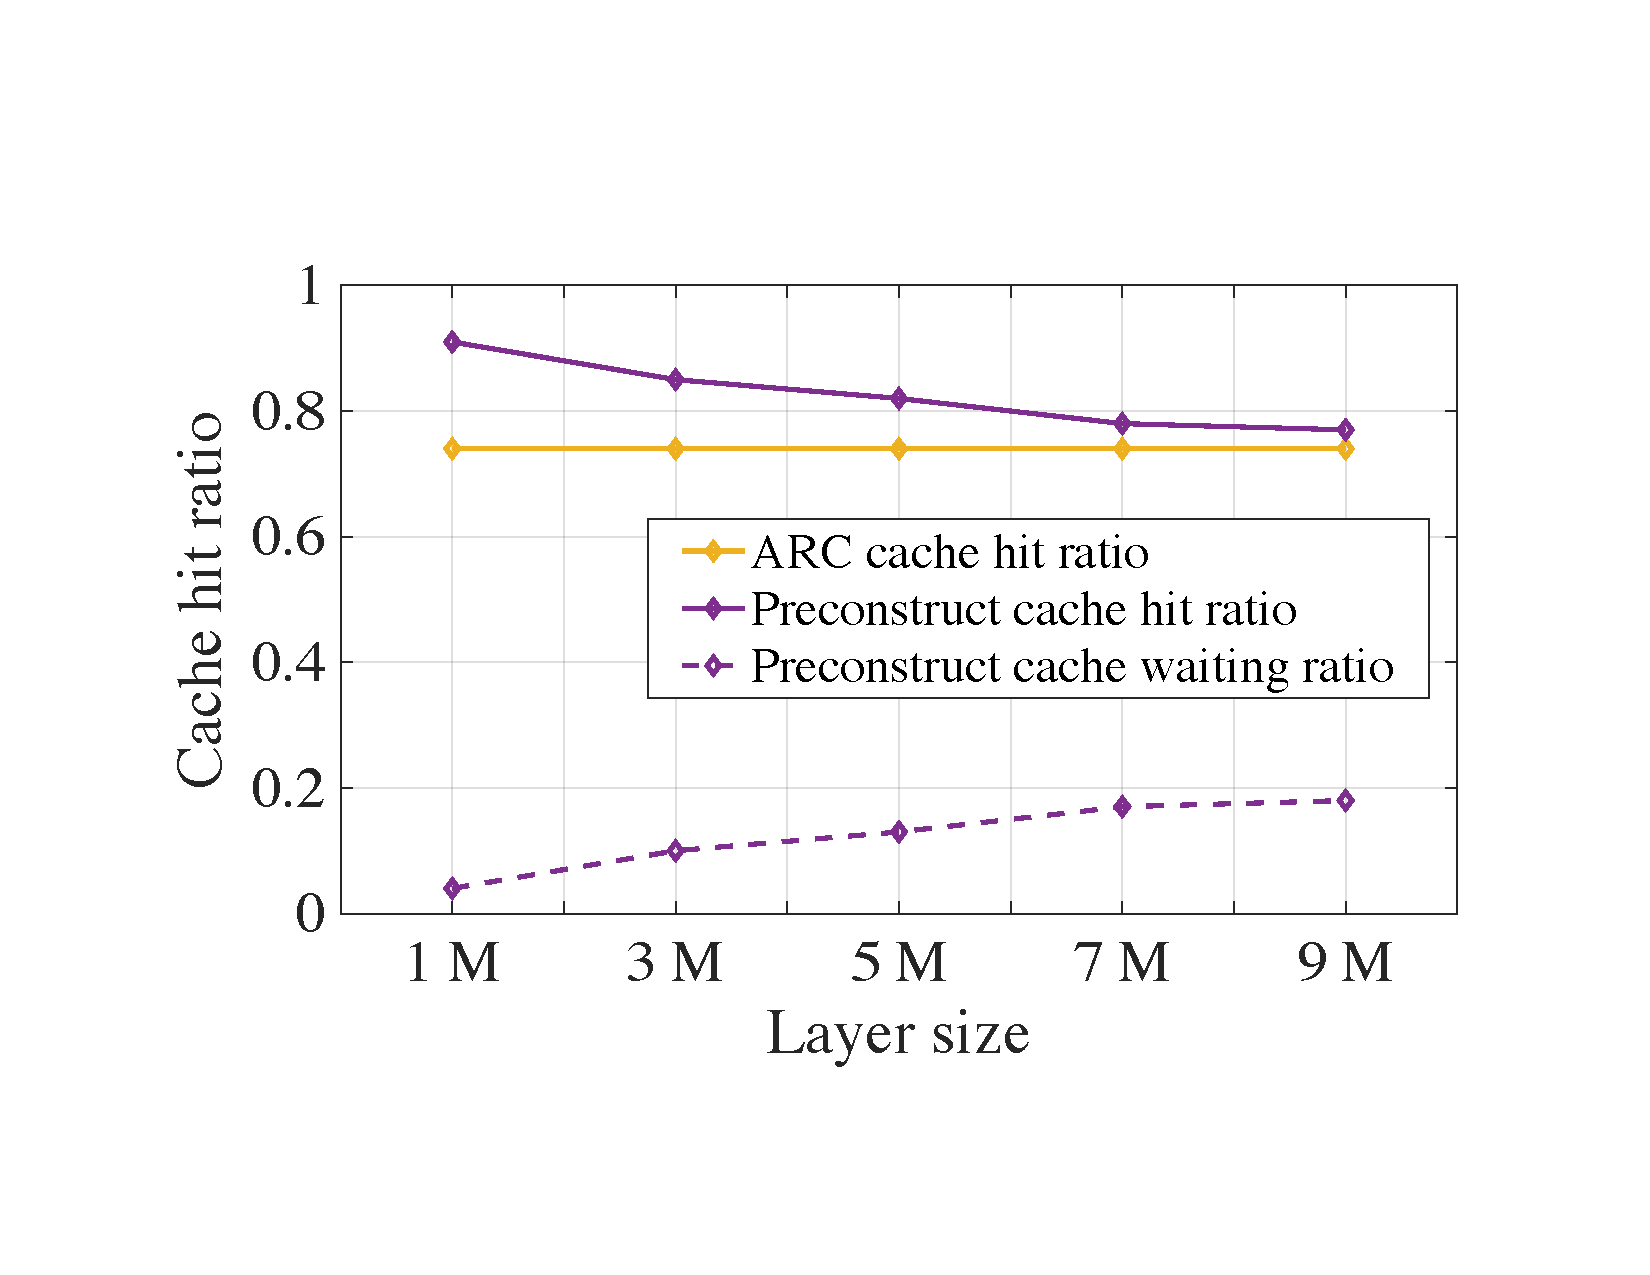
\includegraphics[width=\textwidth]{graphs/cachehitratio.pdf}
		\caption{Cache hit ratio}% of LRU cache and preconstruct cache.}
		\label{fig:eval-cachehitratios}
	\end{minipage}%
\hspace{1mm}
	\begin{minipage}{0.28\textwidth}
	\centering
	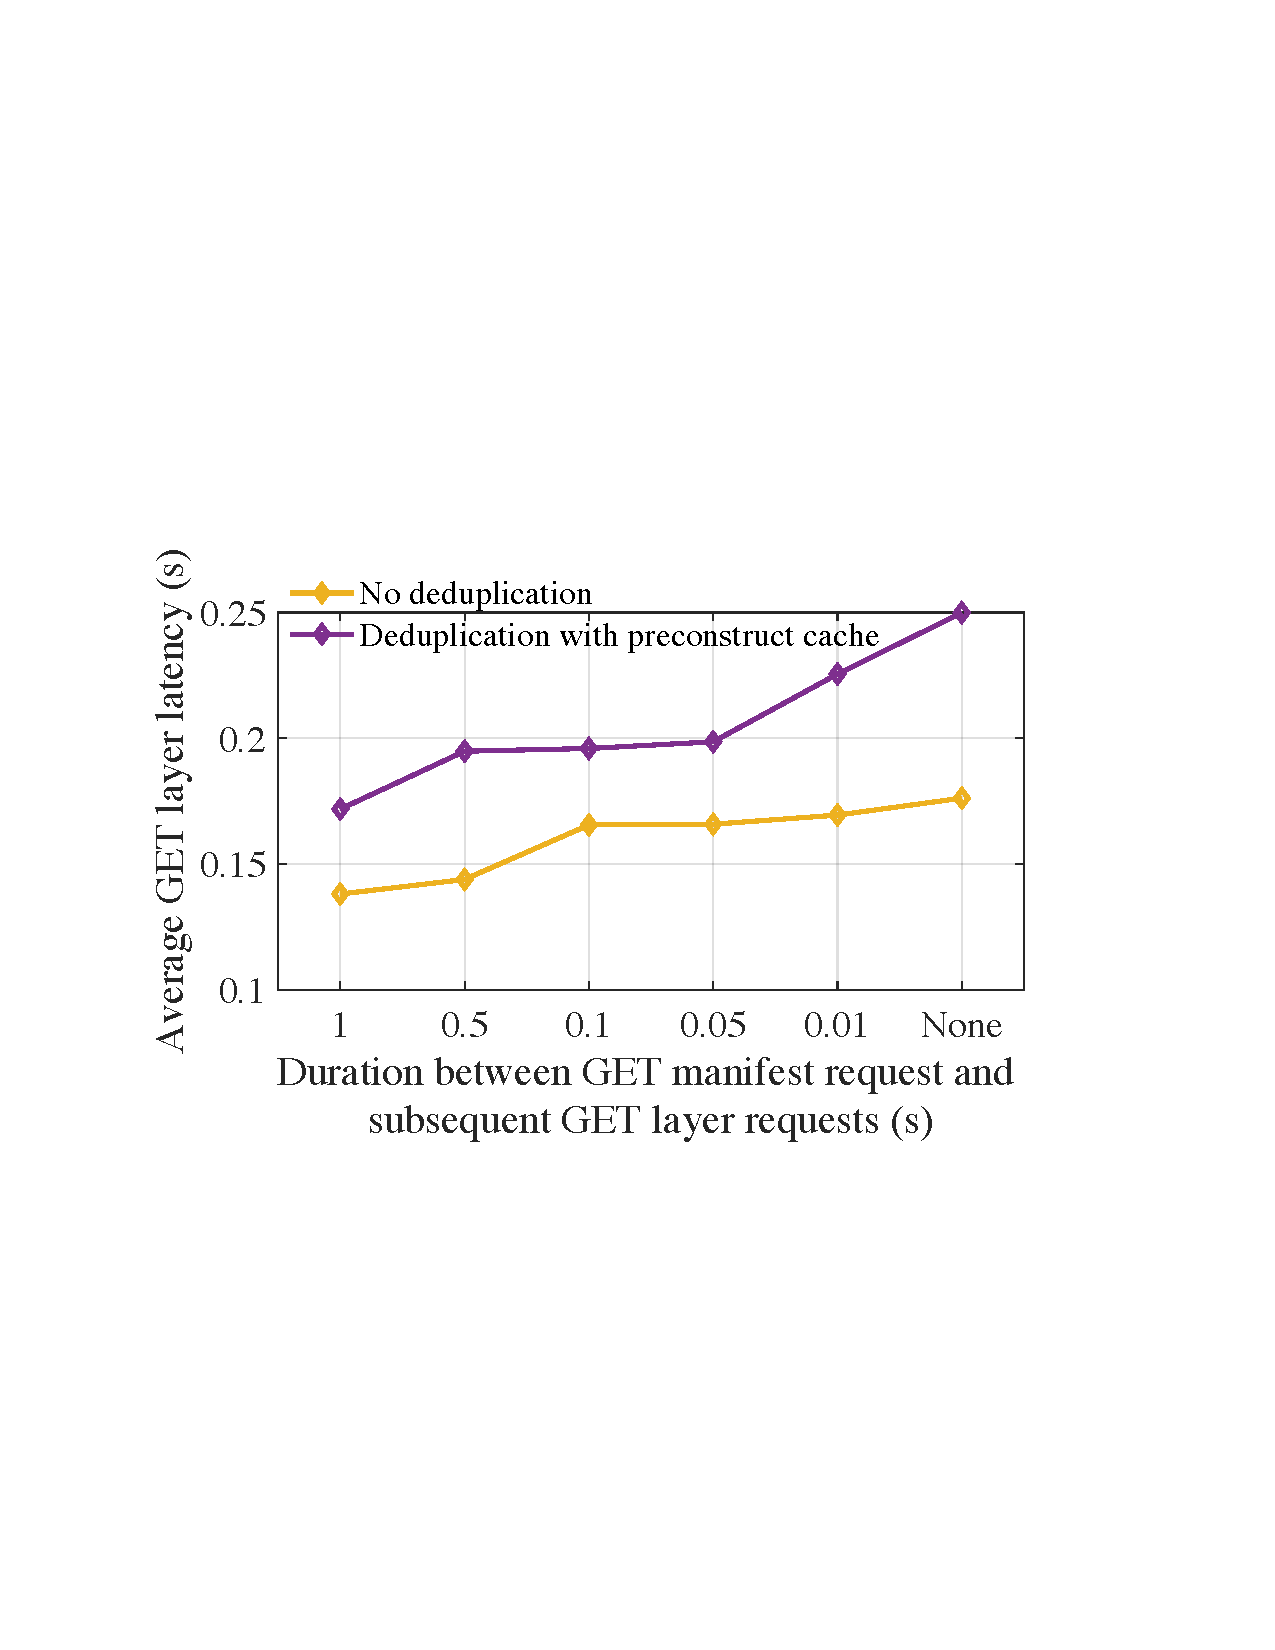
\includegraphics[width=\textwidth]{graphs/durationML.pdf}
	\caption{\texttt{GET} manifest/layer IAT}
	\label{fig:eval-durationML}
   \end{minipage}
\end{figure*}

In this section, we evaluate the layer restoring latency of \sysname's deduplication cluster 
and its impact on \texttt{GET} layer request latency.
%
We first measure a single D-server's layer restoring capability and compare it with 
a \emph{no deduplication} scheme, i.e.  a plain registry server with a local file system backend
that performs no deduplication.
%
Then we scale out to a deduplication cluster with multiple D-servers and compare
\sysname to BOLT~\cite{littley2019bolt}, a recently published, state-of-the-art registry design.
%
%a consistent hashing based distributed docker registry cluster 
%that utilizes the local file systems on the nodes for storage.
%
%
% (denoted as
%\sysname-dedup)
% and 
%overhead of layer deduplication on .
%To measure the  
%We compare the \texttt{GET} layer latency of D-servers
%with 
%by running \sysname with \text{only deduplication} on a single D-server.
%We launch a client on another server and \texttt{pulls} 3 layers in parallel.
%We configure \sysname as
%registry without deduplication,
%deduplication registry,
%deduplication registry with LRU cache~\cite{xxx},
%and
%deduplication registry with a preconstruct cache.
%We set the cache size as 20\% of ingress data.

\paragraph{Restoring latency}
%
%\LR{Why are we only looking at layers between 1 and 9\,MB?}
%\NZ{We start from small layers to big layers like 70 MB.
%small layers can be restored by using just a single node.}
%\LR{Is the ARC cache the layer stage area cache or what does it refer to in Figure 3a?}
%\NZ{No. ARC cache is a layer cache which stores the constructed hot layers
%to save restoring time. ARC cache does not preconstruct layers.}
%
To evaluate \sysname{}'s restoring latency, we launch a single node registry on a server
and use one client on a separate machine.
%
We compare four different configurations:
(1)~no deduplication;
(2)~\sysname without caching;
(3)~\sysname with ARC caching but no preconstruction; and
(4)~\sysname with preconstruct cache.
%
For each setup, we use the local file system as the storage backend and replay the
\dal workload with layer size groups from 1\,MB to 9\,MB. For this experiment, we focus
only on smaller layers as our registry setup is single-node.
%
%\LR{Above we say we match layers randomly?}
%\NZ{yes}
%
%The client matches requests from \dal to layers with similar sizes 
%from the evaluation dataset and replays them to the D-server.
%We compare four backends: 

%\LR{Do we also have percentiles/errorbars or just averages?}
%\NZ{we have 90th percentile.}
%
As shown in Figure~\ref{fig:eval-1nodegetlayerlatency}, 
layer restoring increases the average \texttt{GET} layer request latency by 189\% for layers 
with size 1\,MB for \sysname without caching compared to \emph{no deduplication}.
%
Moreover, the layer restoring latency increases almost linearly as the layer size increases.
%
While a 1\,MB layer takes 0.13\,s to restore and download, 
it takes 0.22\,s for a 9\,MB layer for \sysname without caching.

%\paragraph{Preconstruct cache VS. ARC cache}
%\paragraph{Cache}
%
The results show that
%As shown in Figure~\ref{fig:eval-1nodegetlayerlatency}, 
%the average \texttt{GET} layer request latency increase with the layer size.
leveraging a cache can largely reduce layer restoring latency.
%
When using an ARC cache, the layer restoring overhead decreases by 40\% for layers with
a size of 1\,MB compared to \sysname without cache.
%
However, as the layer size increases,  the improvement drops.
%
For 9\,MB layers, the presence of the ARC cache reduces the average layer restoring overhead by only 16\%
from the overhead of using Sift without caching.
%
%\LR{Do we have a reason for that?}
%\NZ{This is because it takes longer to restore a bigger layer upon a cache miss.}
%
%\Subil{there is no 10-MB value in Fig~\ref{fig:eval-1nodegetlayerlatency}.}
%ARC cache can only improve 10\% of 
%Restoring a layer puts 150\% overhead on \texttt{GET} layer latency.
%By adding a ARC cache,
%he average \texttt{GET} layer latency decreases by 39\%.
With the preconstruct cache, \sysname is able to improve \texttt{GET} layer latencies even further.
%
For 1\,MB layers, the average latency decreases by an additional 24\% compared to the ARC cache.
%
Overall, \sysname with preconstruct incurs the lowest overhead and only increases latencies by
19\% for layers with a 9\,MB size. 

\paragraph{Cache hit ratio}
%
Figure~\ref{fig:eval-cachehitratios} shows the cache hit ratios for the ARC and
preconstruct caches.
%
Note that the cache size is set to 20\% of \dal{}'s ingress data, i.e., 20\% of the total size of
all unique layers, which are pushed to the registry as part of our workload.
%
%\NZ{Here, the cache size = unique layer count x layer size x 0.2.
%Cache size depends on the layer size we chose.
%we replay the workload five times, varying
%the layer size (from 1~MB to 9~MB)
%For example, if layer size is 1 M,
%then the cache size = unique layer count x I MB x 0.2
%= 1278*0.2MB.}
%
%\Subil{approximately how much is Dal's ingress data?}.
%
The cache hit ratio for ARC is stable at 0.77 for all layer sizes while
the preconstruct cache achieves a hit ratio of 0.95 for 1\,MB.

As the layer size increases to 9\,MB, the preconstruct cache hit ratio decreases to 79\%.
%
This is because the layer restoring latency increases with layer size as shown in
Figure~\ref{fig:eval-1nodegetlayerlatency} and therefore, some layers can not be preconstructed
on time.
%
%\LR{We should introduce waiting ratio here.}
%\NZ{The waiting ratio is calculated by the number of \texttt{GET} layer requests that are waiting for
%layer preconstruction process to finish divided by the total number of \texttt{GET} layer requests.}
%
This is indicated by the increasing number of waiting \texttt{GET} layer requests for larger layer
sizes, depicted by the preconstruct cache waiting ratio in Figure~\ref{fig:eval-cachehitratios}.
%
The waiting ratio is the number of \texttt{GET} requests that were blocked on reconstruction
divided by the total number of \texttt{GET} requests.
%
%Since layer construction already starts before these requests arrive, the restoring overhead can
%be reduced.
%
%\LR{The below is confusing, why is it the sum of the two?}
%\NZ{Its because prediction accuracy is calculated by the number of correct predictions divided by 
%total \texttt{GET} layer requests.
%The \texttt{GET} layer requests that are waiting for preconstruction to finish are also correct predictions.}
%
The user-behavior based request prediction accuracy is calculated by summing the preconstruct
cache hit ratio and the waiting ratio, i.e. all requests that successfully retrieved layers from the cache,
which results to 0.95.
%
%As shown in Figure~\ref{fig:eval-cachehitratios}, the prediction accuracy is 0.95.

\begin{figure*}[t]
	\centering
	\begin{minipage}{0.3\textwidth}
		\centering
		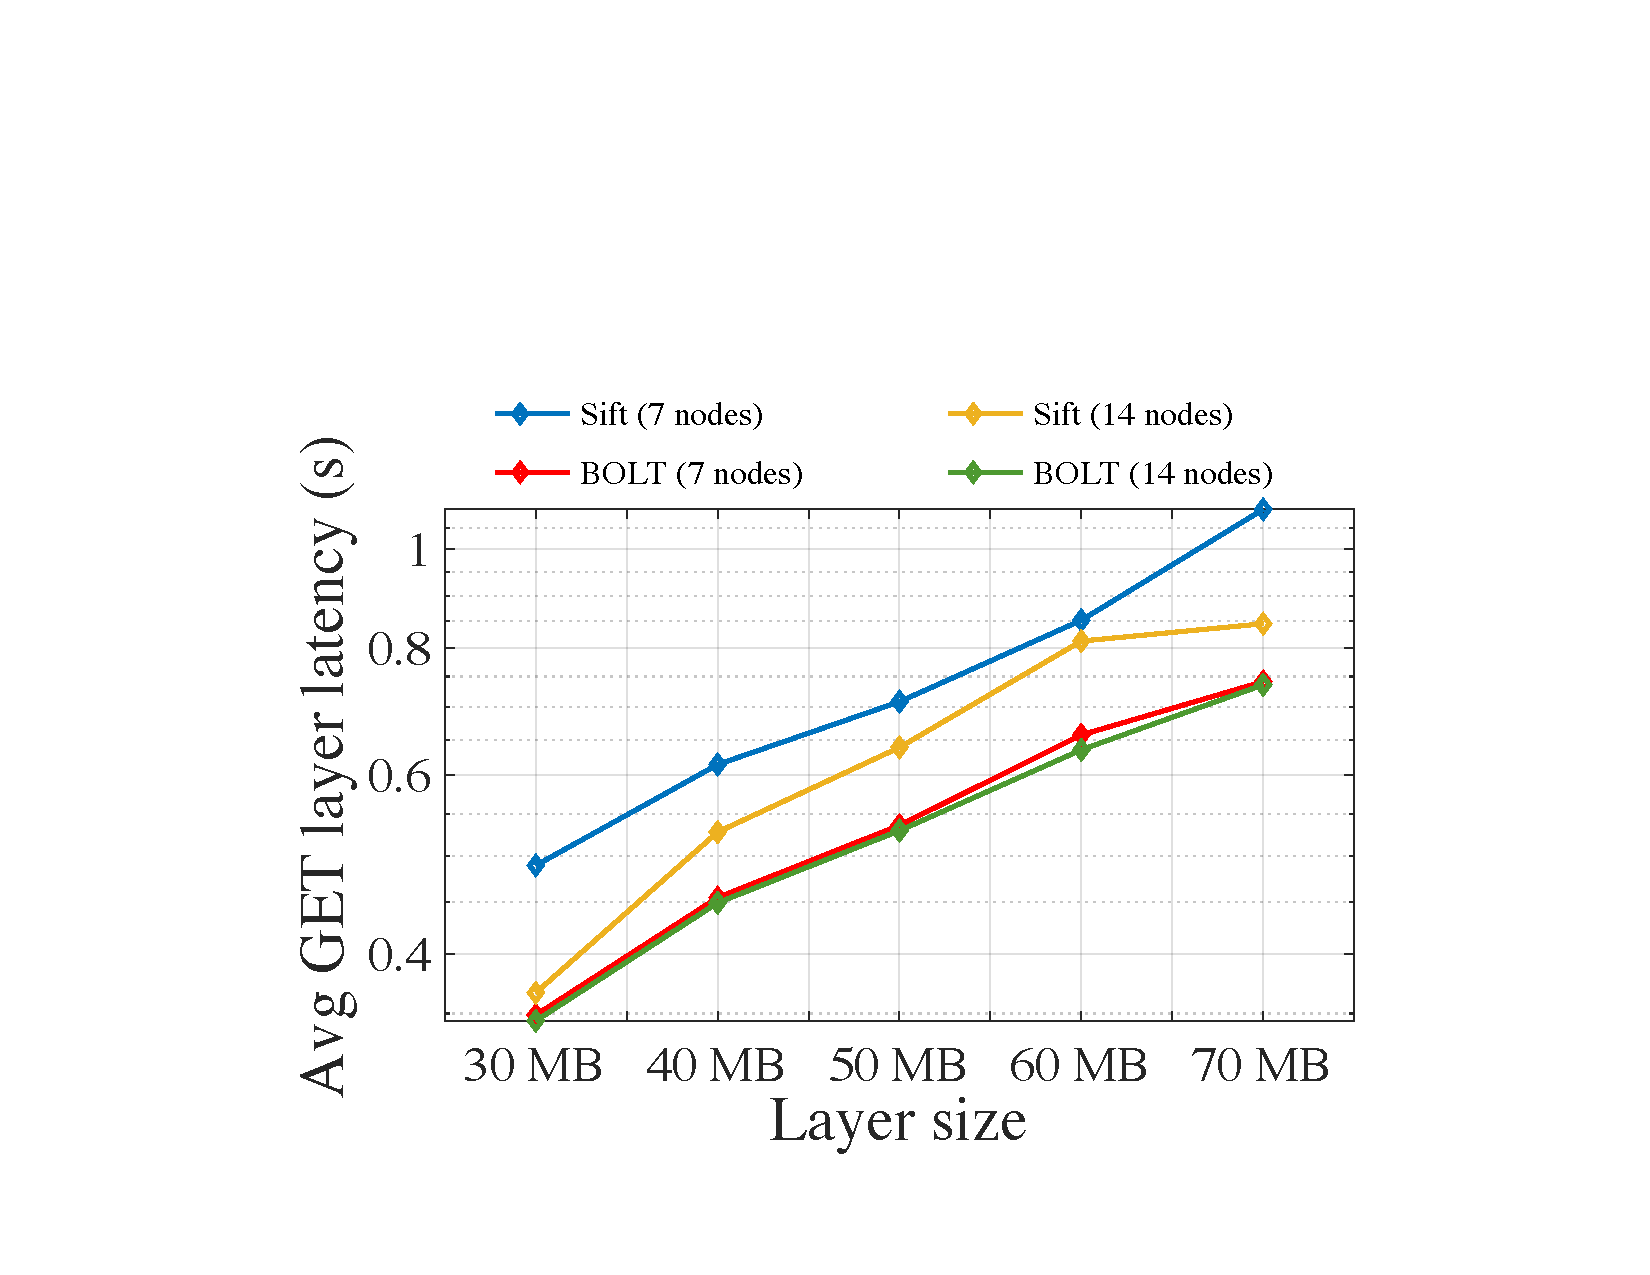
\includegraphics[width=\textwidth]{graphs/clusterscale.pdf}
		\caption{GET layer latency with different cluster size}
		\label{fig:eval-clusterscale}
	\end{minipage}%
	\hspace{1mm}
		\begin{minipage}{0.3\textwidth}
		\centering
		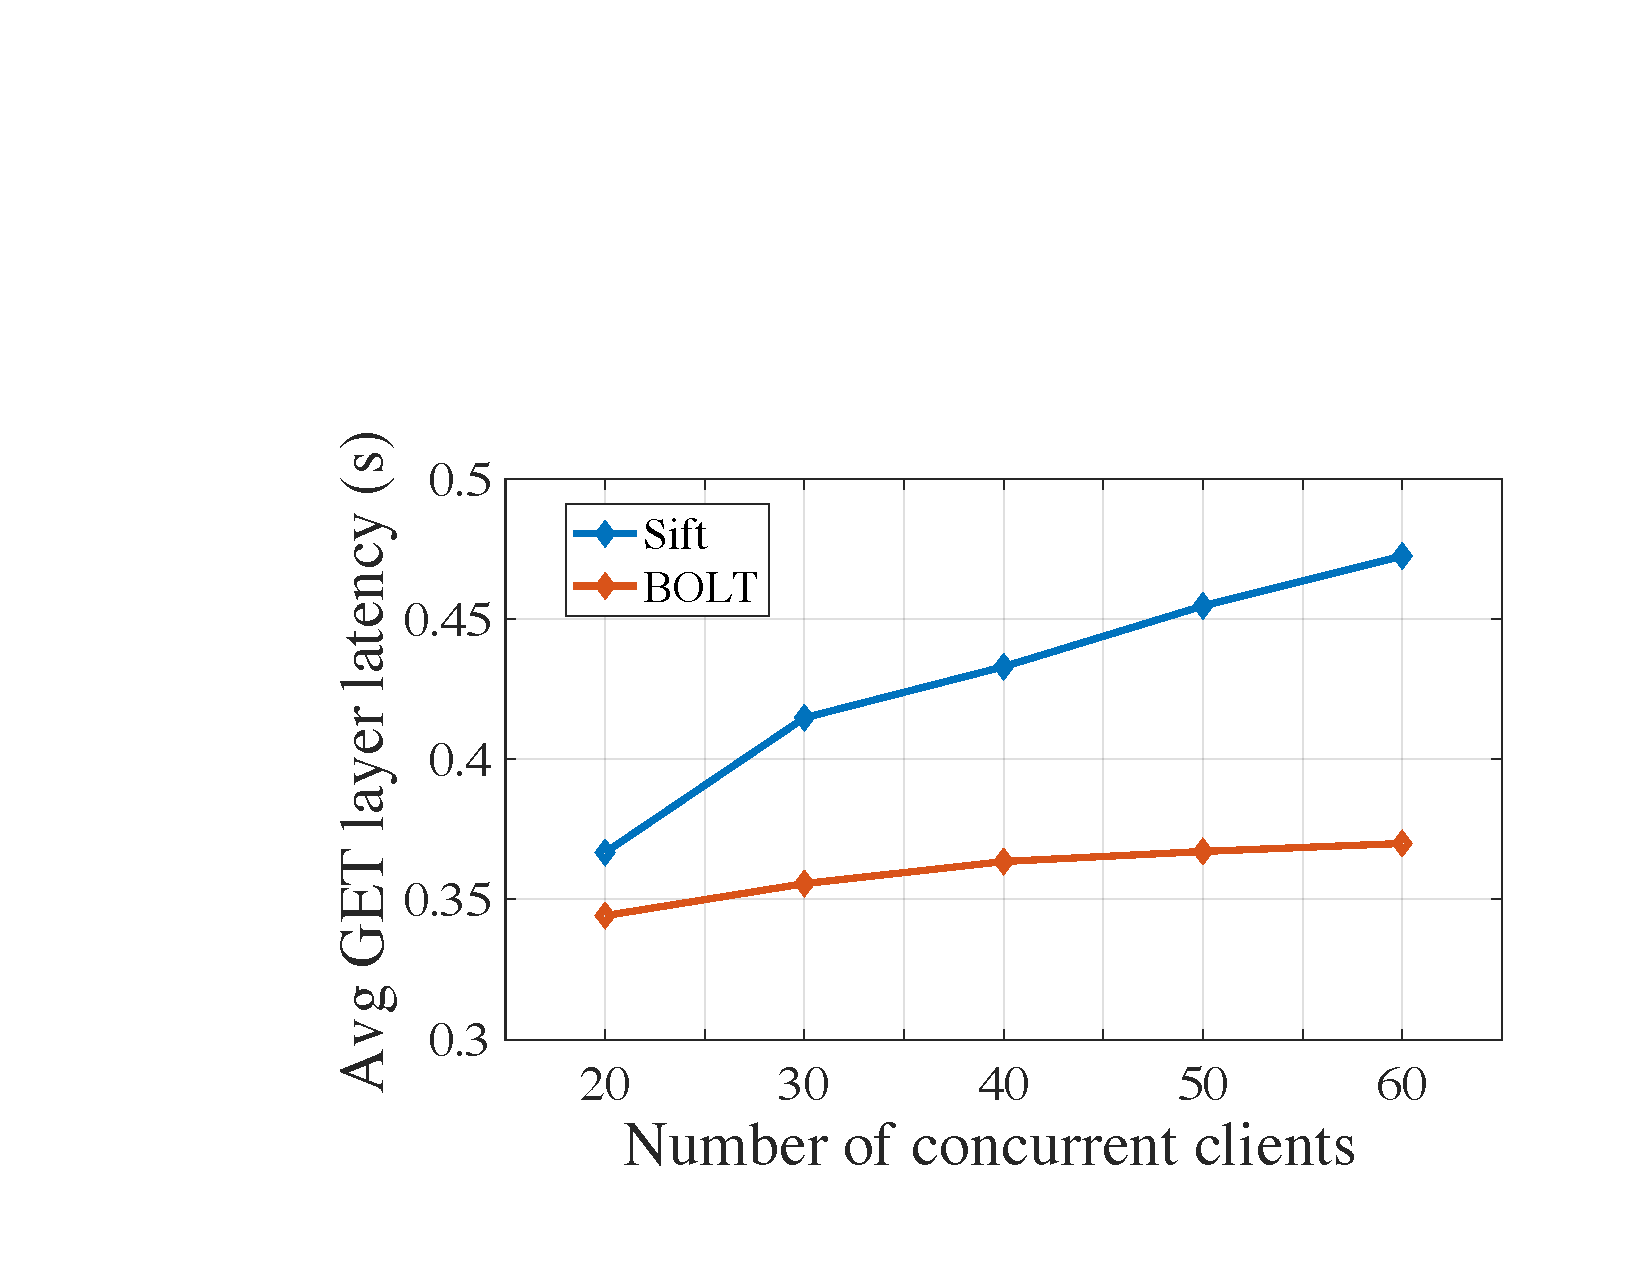
\includegraphics[width=\textwidth]{graphs/clientscale.pdf}
		\caption{GET layer latency with different client concurrency}
		\label{fig:eval-clientscale}
	\end{minipage}%
	\hspace{1mm}
	\begin{minipage}{0.3\textwidth}
	\centering
	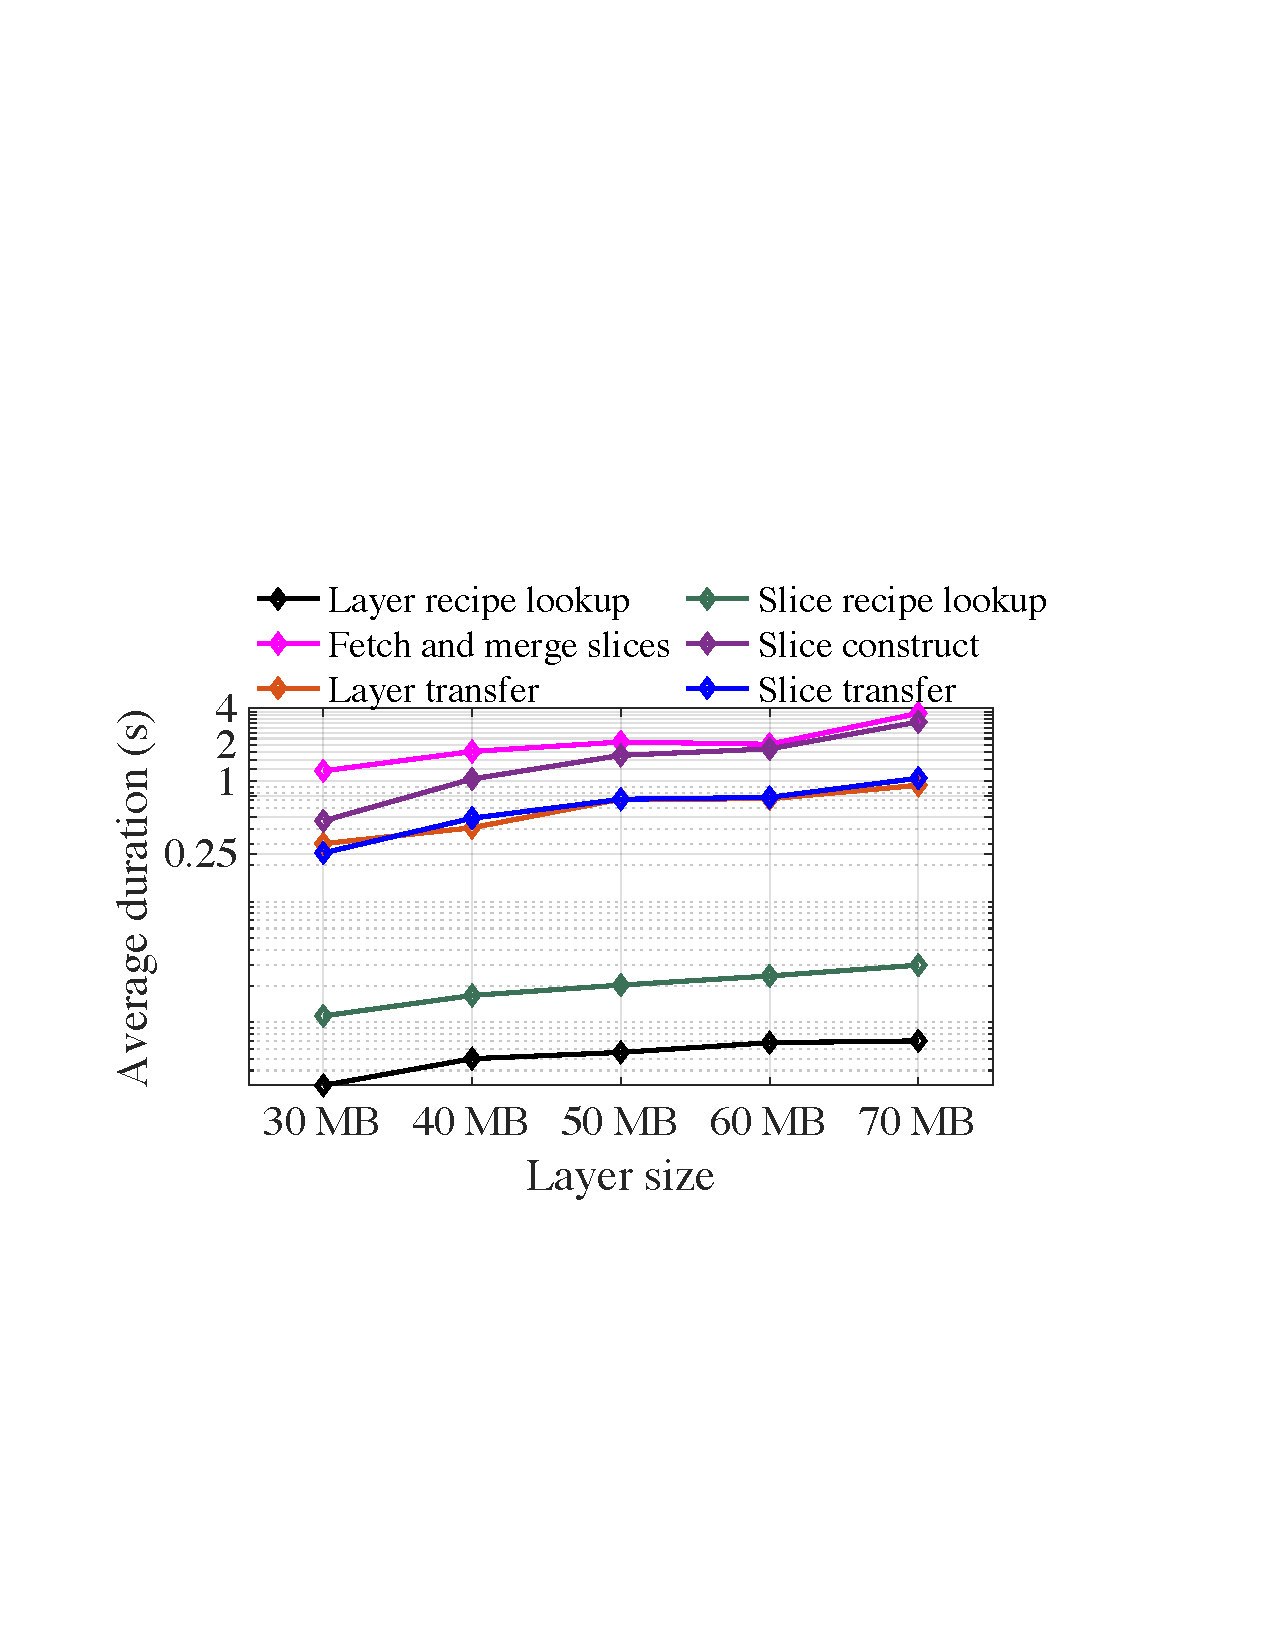
\includegraphics[width=\textwidth]{graphs/restoringbreakdown.pdf}
	\caption{Restoring latency breakdown}
	\label{fig:eval-restoringbreakdown}
	\end{minipage}
\end{figure*}

\begin{figure*}[t]
	\centering
	\begin{minipage}{0.3\textwidth}
		\centering
		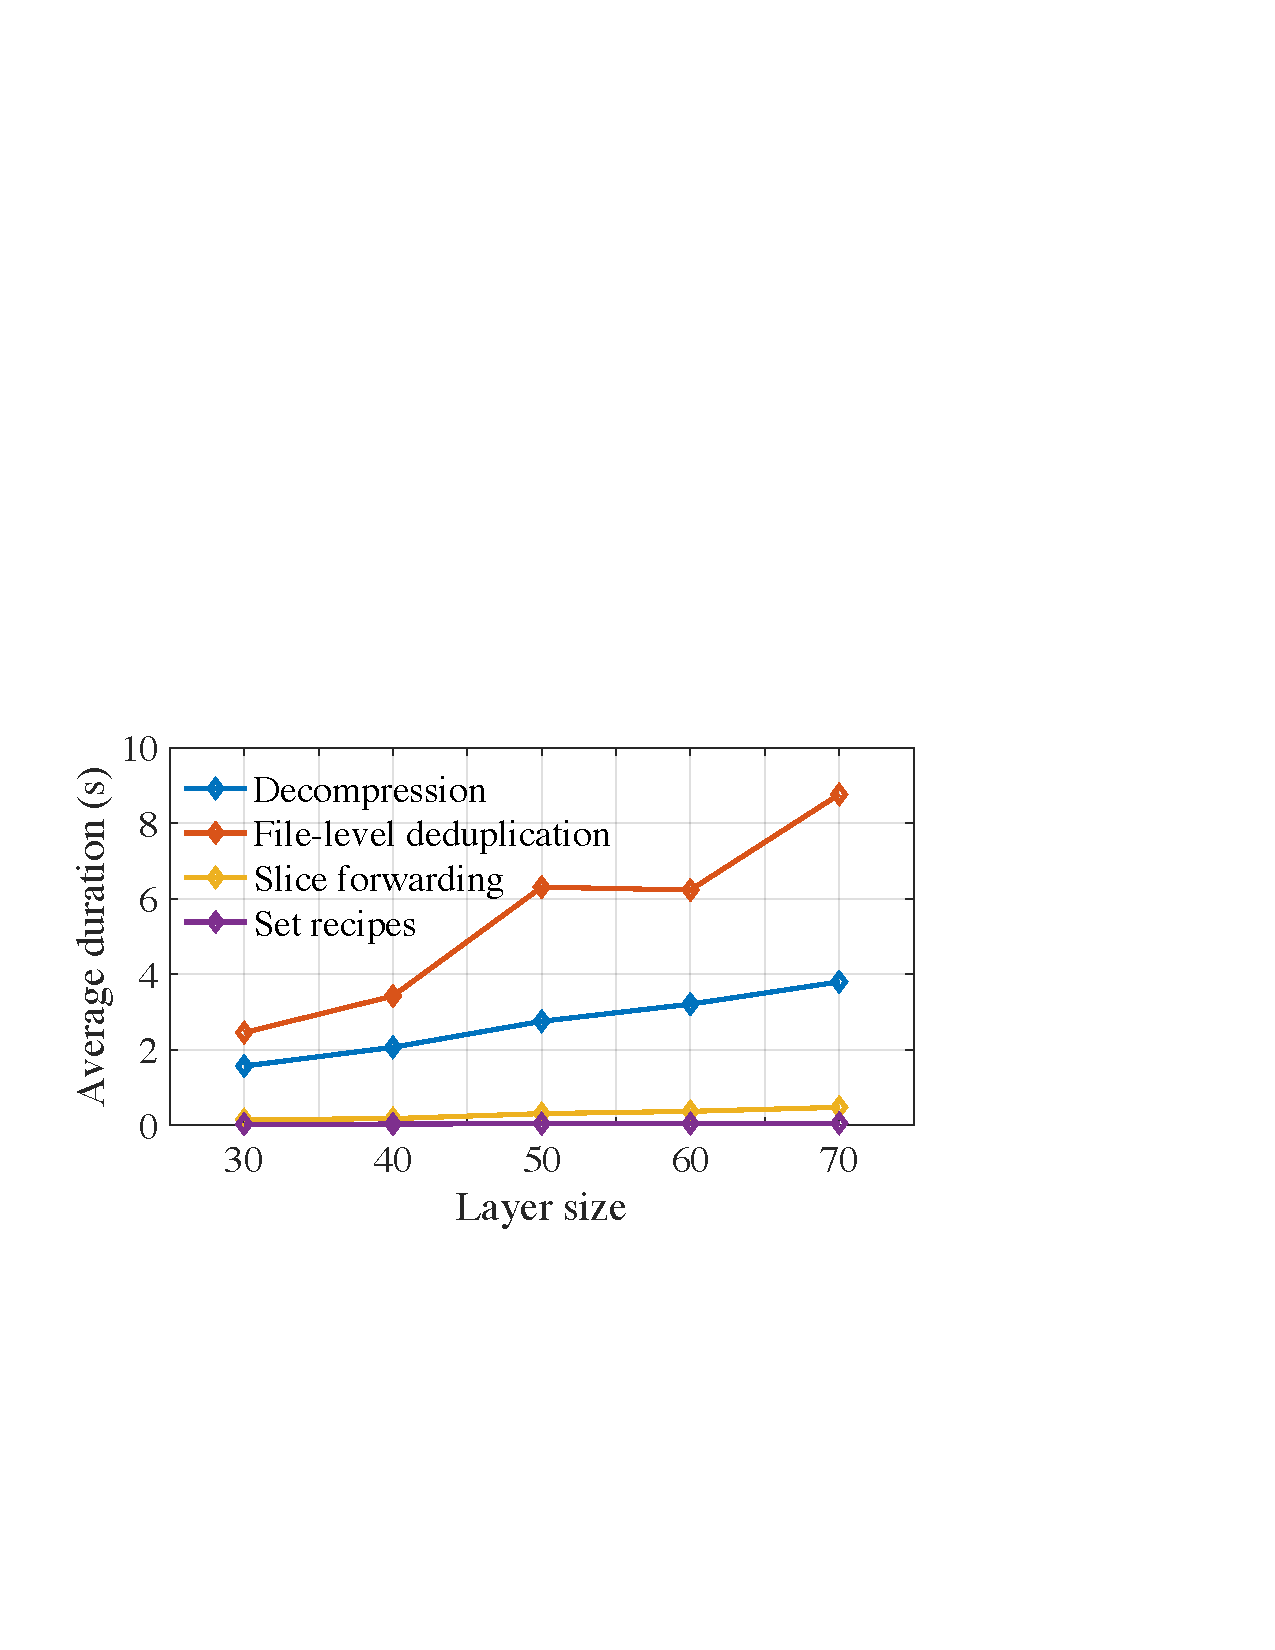
\includegraphics[width=\textwidth]{graphs/dedupbreakdown.pdf}
		\caption{Deduplication latency breakdown}
		\label{fig:eval-dedupbreakdown}
	\end{minipage}%
	\hspace{1mm}
	\begin{minipage}{0.3\textwidth}
		\centering
		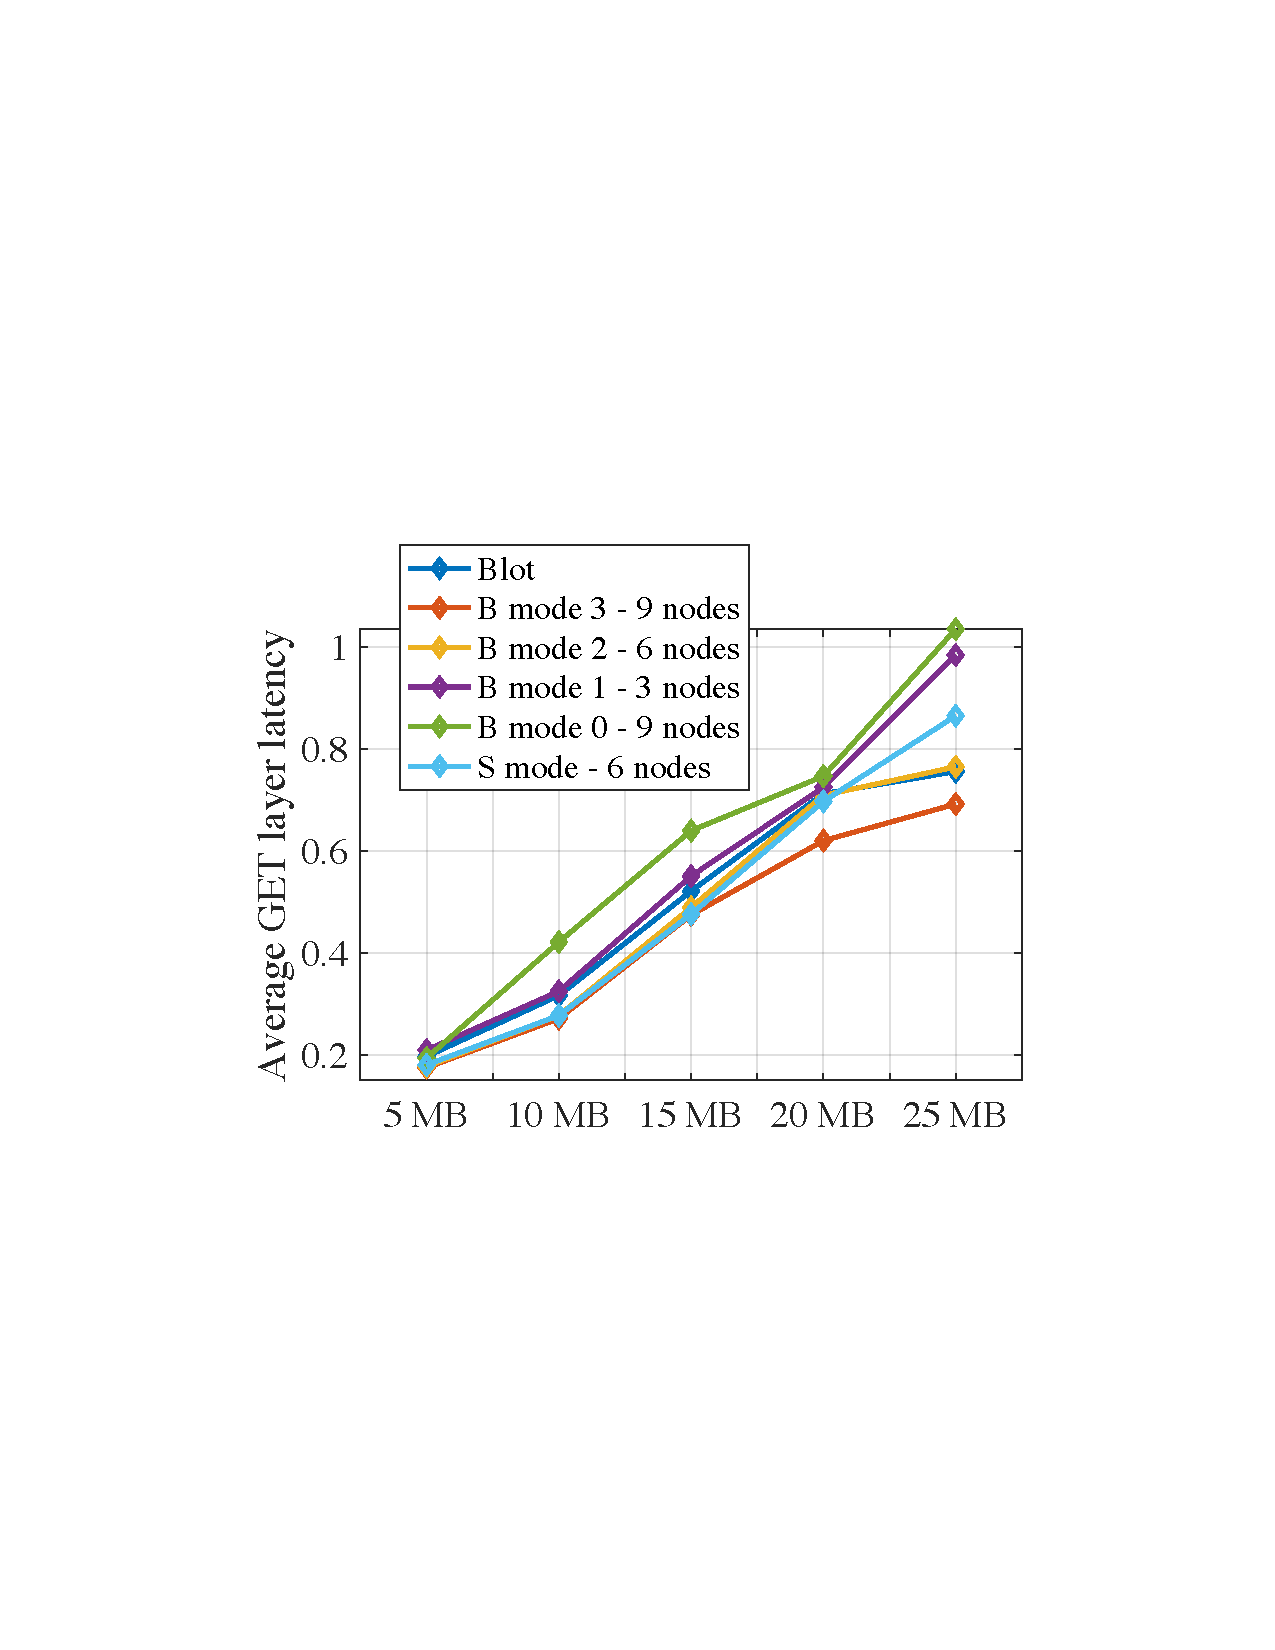
\includegraphics[width=\textwidth]{graphs/dalprimary.pdf}
		\caption{\texttt{GET} layer latency for different layer sizes}
		\label{fig:eval-dalprimary}
	\end{minipage}%
	\hspace{1mm}
	\begin{minipage}{0.3\textwidth}
		\centering
		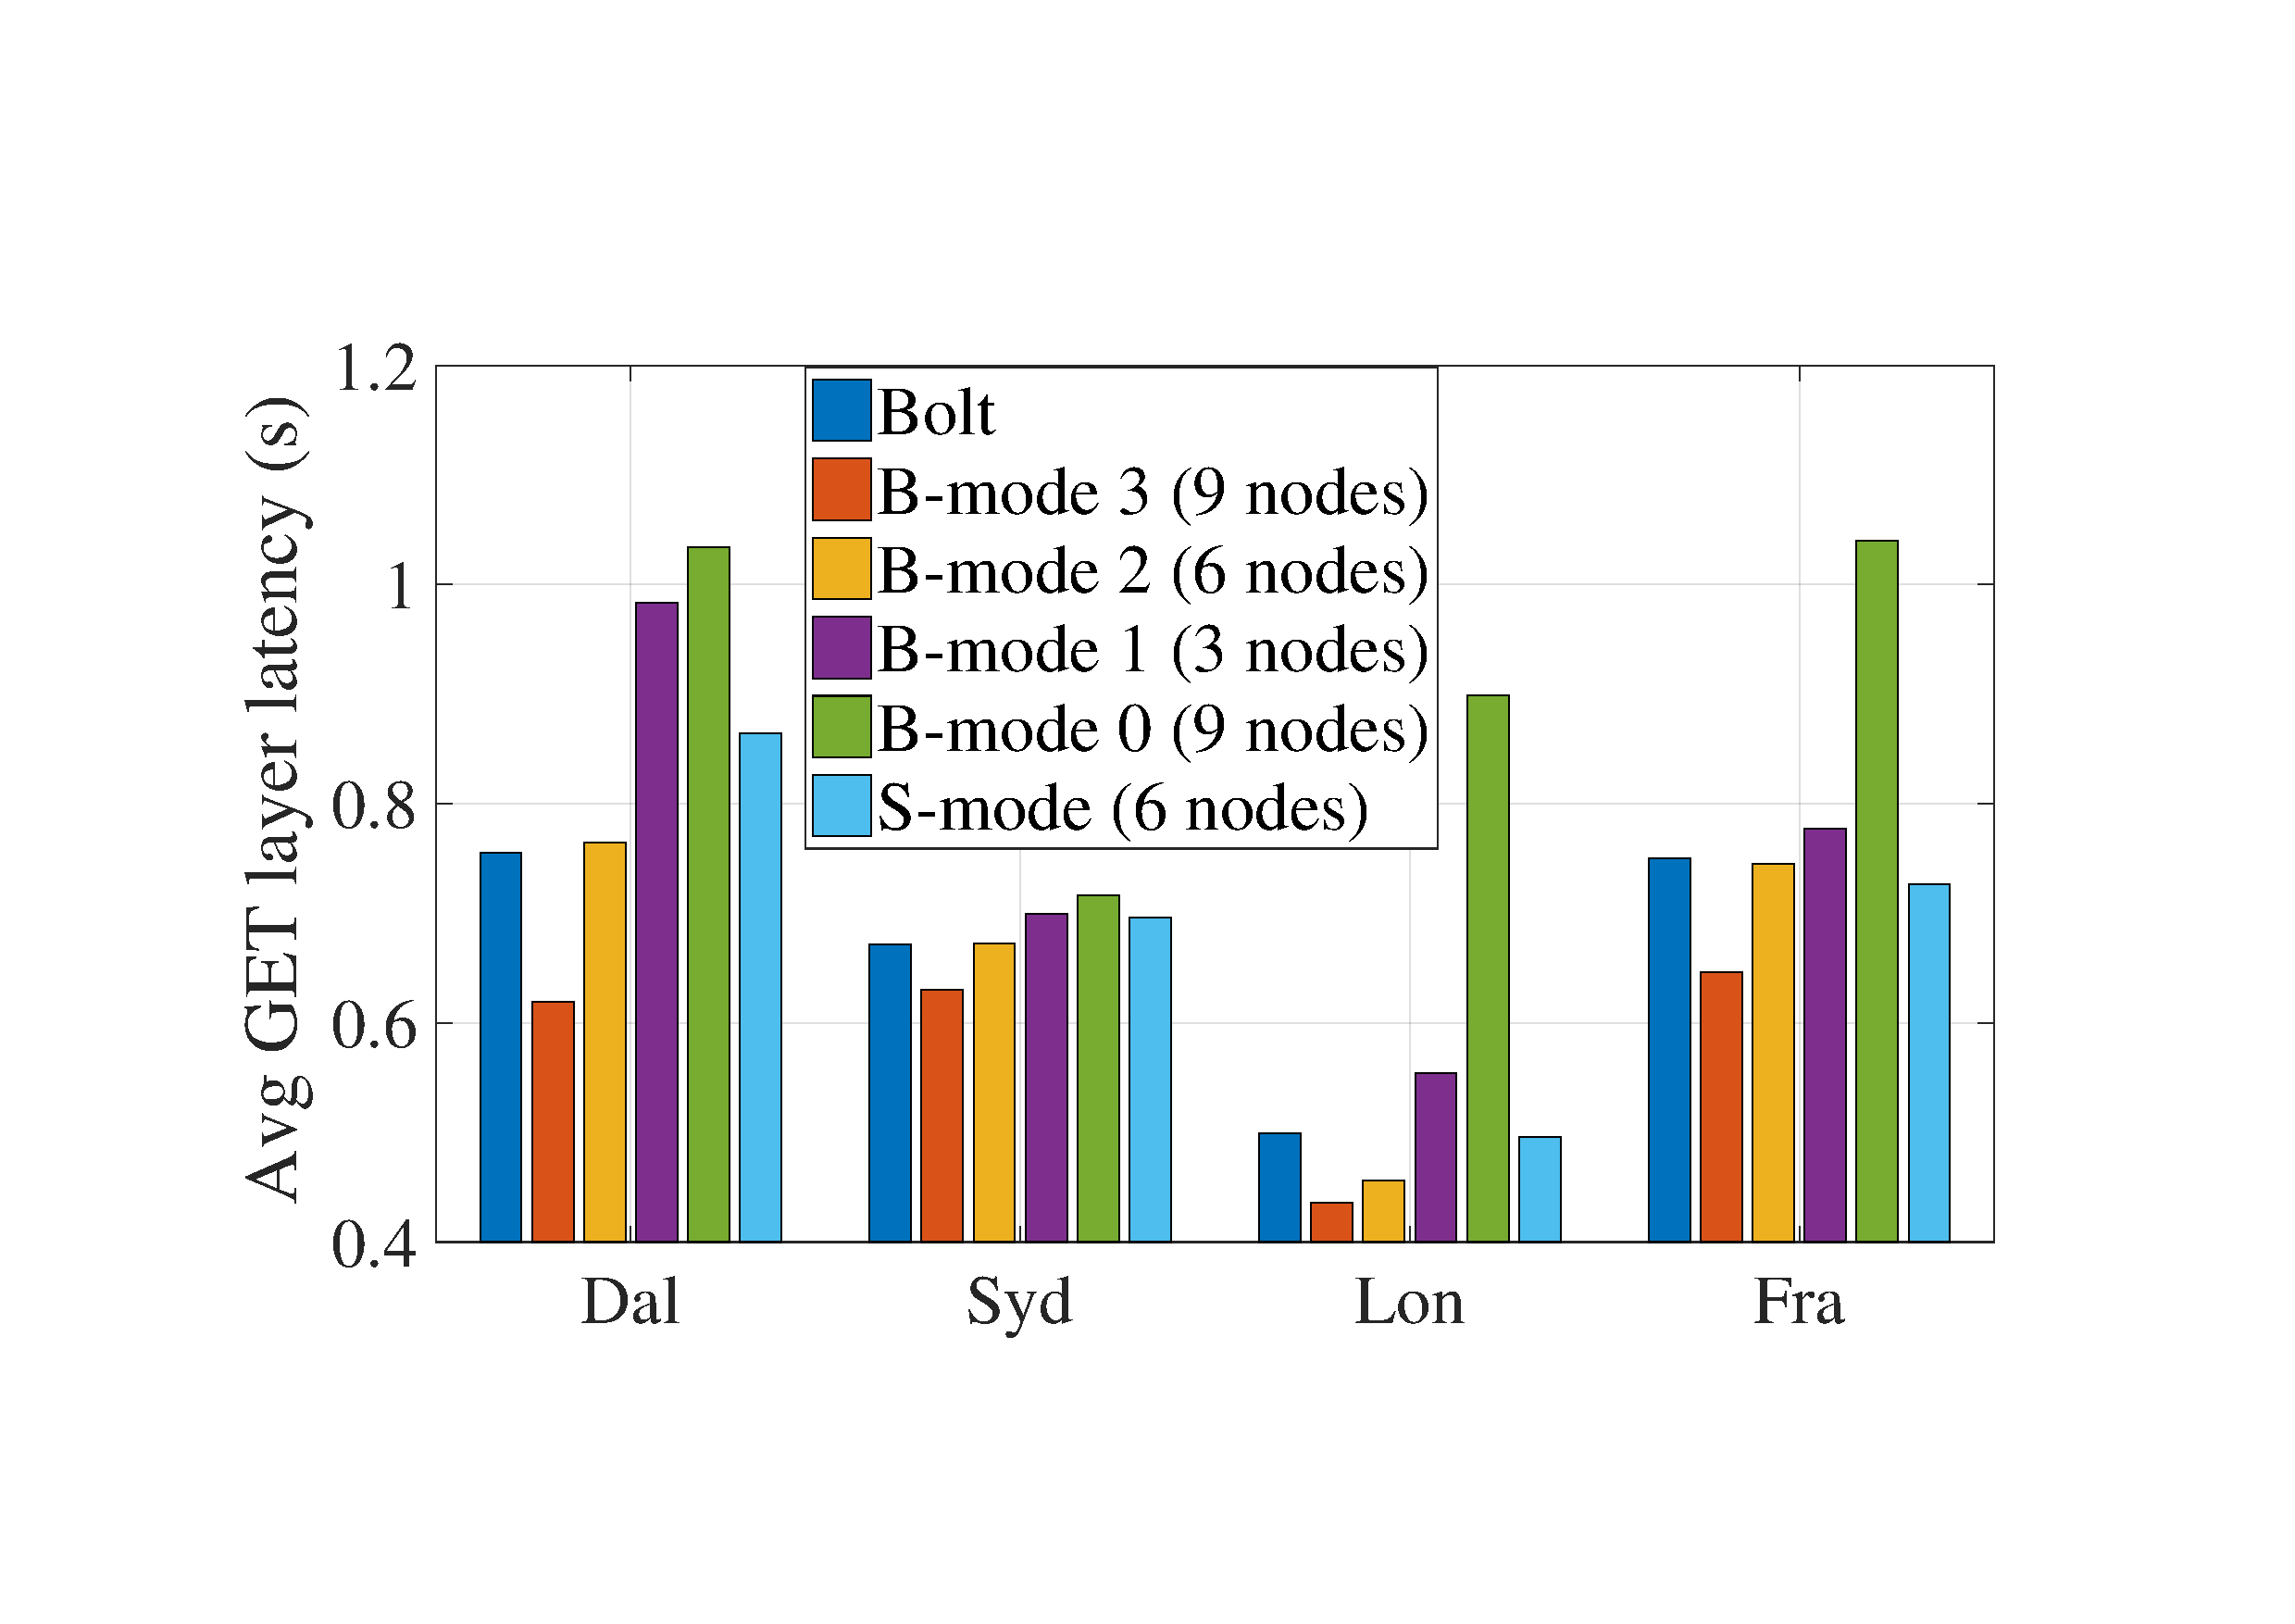
\includegraphics[width=\textwidth]{graphs/total-traces.pdf}
		\caption{\texttt{GET} layer latency for different workloads} %\Subil{"Blot" in figure should be "BOLT".}}
		\label{fig:eval-total-traces}
	\end{minipage}
\end{figure*}
 
\paragraph{Inter-arrival time of manifest and layer requests}
%
Next, we vary the inter-arrival time (IAT) between a \texttt{GET} manifest request and its
subsequent \texttt{GET} layer requests.
%
The layer size used here is 9~MB.
%
Figure~\ref{fig:eval-durationML} compares the average \texttt{GET} layer latency for
\sysname with preconstruct cache versus no deduplication.

When the IAT is 1\,s, \sysname with preconstruct cache only imposes a 19\% overhead.
%
However, as the IAT decreases, the average \texttt{GET} layer latency increases because
layers are not preconstructed in time.
%
When the client replays requests as fast as possible, the overhead of restoring layers on
\texttt{GET} layer requests increases by 30\%.
%
%\LR{How did we replay them in the previous experiment? As fast as possible or downsampled or in
%real-time?}
%\NZ{
%	First, there is an interval or delay between every two subsequent requests.
%	For \texttt{GET} manifest requests, we replay as fast as possible without delay.
%For \texttt{GET} layer requests,
%we use their real intervals if the intervals are smaller than 1 s. Otherwise,
%we use 1 s as the interval.
%We use the above method to replay traces for other tests (not for this different IAT test),
%This is for finishing all evaluations in a reasonable time.}

%the cache hit ratio of the ARC cache and the preconstruct cache.

\paragraph{Cluster scale out}
%
We analyze the impact of larger clusters and layers by increasing the number of registry servers from
7 to 14, and the layer sizes from 30 to 70\,MB and compare \sysname to the BOLT registry.
%
%(1) \sysname deduplication cluster (denoted as \sysname-dedup),
%and
%(2) BOLT \cite{littley2019bolt}.
Each registry server uses the local file system to store, and in the case of \sysname, deduplicate layers.
%
Similarly to BOLT, the consistent hashing logic is implemented at the client
side (see~\S\ref{sec:impl}) to route requests to the correct registry server.
 %Besides, 
 %that the client distributes layers to 
%Therefore,
%we also use our client to cluster the non-dededuplication registry servers and setup BOLT for evaluation.
We launch 20 clients on 2 servers to replay requests to the registries.

As shown in Figure~\ref{fig:eval-clusterscale}, BOLT achieves stable request latencies when
the number of registry servers increases.
%
While \sysname performs worse than BOLT, its performance improves with a larger cluster size.
%
This is because with a bigger deduplication cluster, layers can be restored faster due to higher
parallelism.
%
For example, for a layer size of 30\,MB, doubling the cluster size reduces the restoring
overhead by 35\%.

\paragraph{Workload scale up}
%
Next, we evaluate \sysname{}'s performance for an increasing workload.
%
We vary the number of concurrent client requests and measure the average \texttt{GET} layer
request latency on a 14-node cluster for \sysname and BOLT.
%
The results are shown in Figure~\ref{fig:eval-clientscale}.

BOLT only experiences a slight increase in \texttt{GET} layer latency as the number of clients increase.
%
On the other hand, latencies for \sysname increase linearly with the number of concurrent client requests.
%
For example, for 20 concurrent requests, the average \texttt{GET} layer latency is 0.37\,s which
increases to 0.47\,s for 60 concurrent requests.
%
This is because layer restoring is computationally intensive, i.e. for more concurrent requests, the CPU
becomes a bottleneck.

\paragraph{Restoring latency breakdown}
%
To analyze \sysname{}'s performance in more detail, we measure the time it takes
to reconstruct a layer and break the process down into its individual steps.
%
The steps in layer reconstruction include looking up the layer recipe, fetching and merging 
slices, and transferring the layer. Fetching and merging slices in itself involves slice recipe 
lookup, slice construction, and slice transfer.
%
%\LR{This is unclear, we've never talked about complete or waiting restoring processes before.
%What exactly are we doing here?}
%\NZ{We can delete "complete or waiting restoring processes" if it's confusing.
%"complete restoring processes" means the \texttt{GET} layer request misses on cache without
%layer preconstruction to wait.
%So this layer restoring process will have all the steps shown in  Figure~\ref{fig:eval-restoringbreakdown}.
%We count them in the figure.
%"waiting restoring processes" means the \texttt{GET} layer request misses cache but the request waits because
%layer preconstruction hasn't finished yet.
%So this layer restoring process will not have layer construct step. Instead it has a waiting step.
%We don't count them in the figure.
%Except for the above \texttt{GET} layer requests,
%we have \texttt{PRECONSTRUCT} layer requests.
%Those requests also initiate layer restoring processes, which contains all steps shown in
%Figure~\ref{fig:eval-restoringbreakdown}.
%We count them in the figure.}
%
%We only include complete layer restoring processes and eliminate the layer restoring processes
%that are waiting for others to construct layers.
%
%\LR{Again, the following is confusing. What does it mean?}
%\NZ{we count the layer restoring processes for both \texttt{GET} layer requests and
%\texttt{PRECONSTRUCT} layer requests.}
%
%Note that the layer restoring latencies measured also include layer restoring processes for preconstruction.
%
The latencies are measured on the 7-node cluster and the breakdown is shown in
Figure~\ref{fig:eval-restoringbreakdown}.

We can see that slice reconstruction accounts for the largest portion of layer construction time.
%
Slice construction involves file archiving and compression, which are the main bottlenecks.
%. 
Layer construction time increases with layer size because layer slices become bigger and
take longer to archive and compress.
%
For example, for layers of size 30\,MB, fetching and merging slices takes 1.3\,s on average while
for 70\,MB layers, it takes 3.6\,s.

\paragraph{Deduplication latency breakdown}
%
Finally, we study the deduplication process in more detail.
%
Note that to reduce the impact of layer deduplication on the \texttt{GET} layer request,
the layer deduplication process runs in off-line mode.
%
Figure~\ref{fig:eval-dedupbreakdown} shows the breakdown of the deduplication latency.

We observe that decompression and file-level deduplication account for the largest portions of
the layer deduplication duration.
%
%\LR{Why does the following reduce the overhead? Do we want to reduce the impact on the
%restoring processes?}
%\NZ{Because there are \texttt{GET} and \texttt{PUT} requests.
%We configure deduplication process to use a single thread to 
%minimize its computation and I/O resource consumption
%so it wont compete for resources with layer restoring process. }
%
This is because \sysname uses single-threaded decompression and file-level deduplication in
order to reduce interference with the critical layer restoration processes.
%
%\Subil{This conflicts with our description of pgzip in the Implementation section where we
% talk about using parallelism in both compression ad decompression}.
%\NZ{pgzip is for layer restoring. We use standard gzip for deduplication.}
%\Subil{Since we are only using pgzip for compression for layer restoring for pulls and standard
%gzip for decompression during a push, we should remove the implication that pgzip is used
%for both compression and decompression at the end of section 5.2}
%
Moreover, the duration of decompression and file-level deduplication increases with layer sizes.
%
For example, when the layer size increases from 30\,MB to 70\,MB, 
the decompression duration increases from 1.6\,s to 3.8\,s on average and the file-level deduplication duration increases from 2.5\,s to 8.8\,s on average.
%
This is expected as more data needs to be processed.
%\paragraph{Metadata size} 
%Figure~\ref{xxx} shows the average metadata size on each registry server measured by using the size of the used memory in Redis~\cite{redis} when in \emph{B-mode 0}.
%Note that the replication level for the Redis cluster is also set to three.
%As shown, for all traces, the total size of the metadata generated by \sysname such as \emph{recipes} for layers or slices, \emph{indexes} of layers or files, and RLmap or ULmap is less than 100 MB.
%With the 16 GB memory on each registry server, such metadata size is negligible.




%\begin{figure}[t]
%	\centering
%	\begin{minipage}{0.28\textwidth}
%		\centering
%		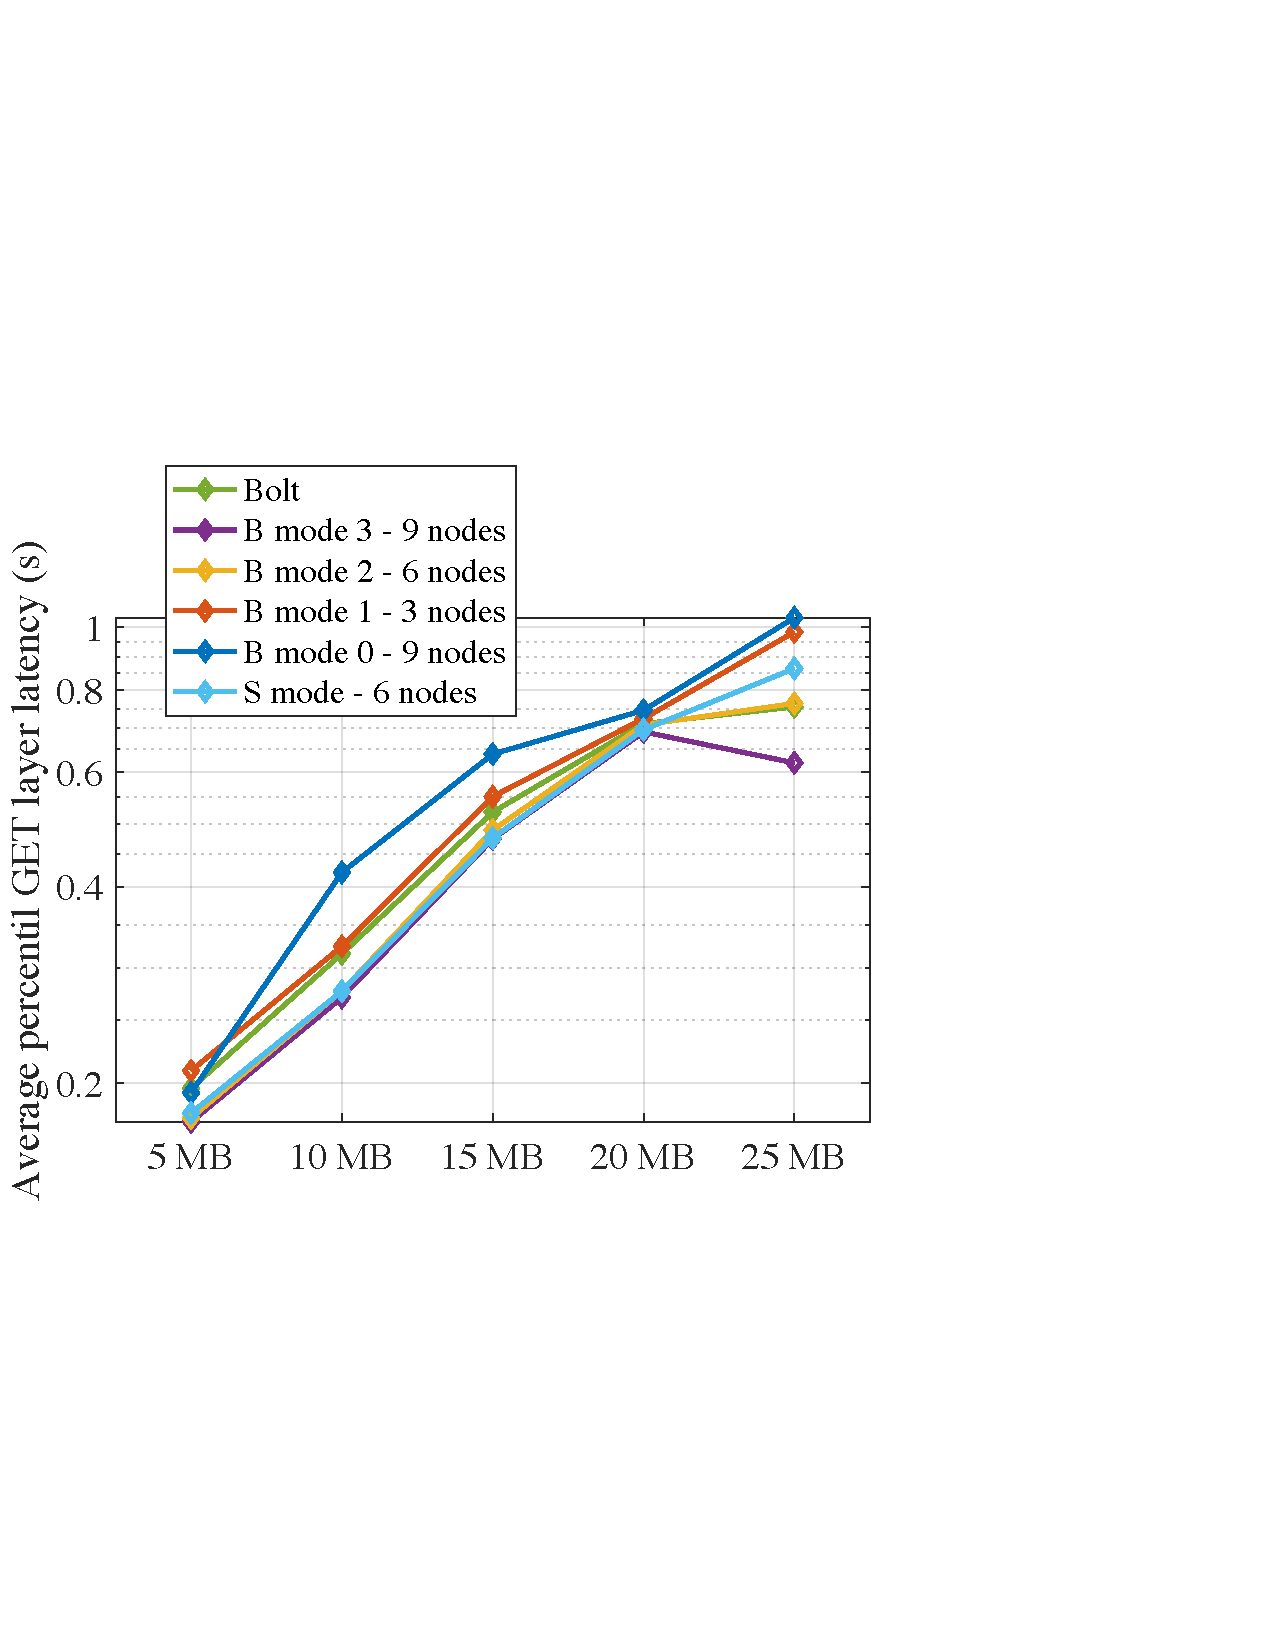
\includegraphics[width=0.9\textwidth]{graphs/dalprimaryperformance.pdf}
%		\caption{GET layer latency.\todo{add grid in background to match the other figures}}% across different schemes.}
%		\label{fig:eval-1nodegetlayerlatency}
%	\end{minipage}%
%	\begin{minipage}{0.28\textwidth}
%		\centering
%		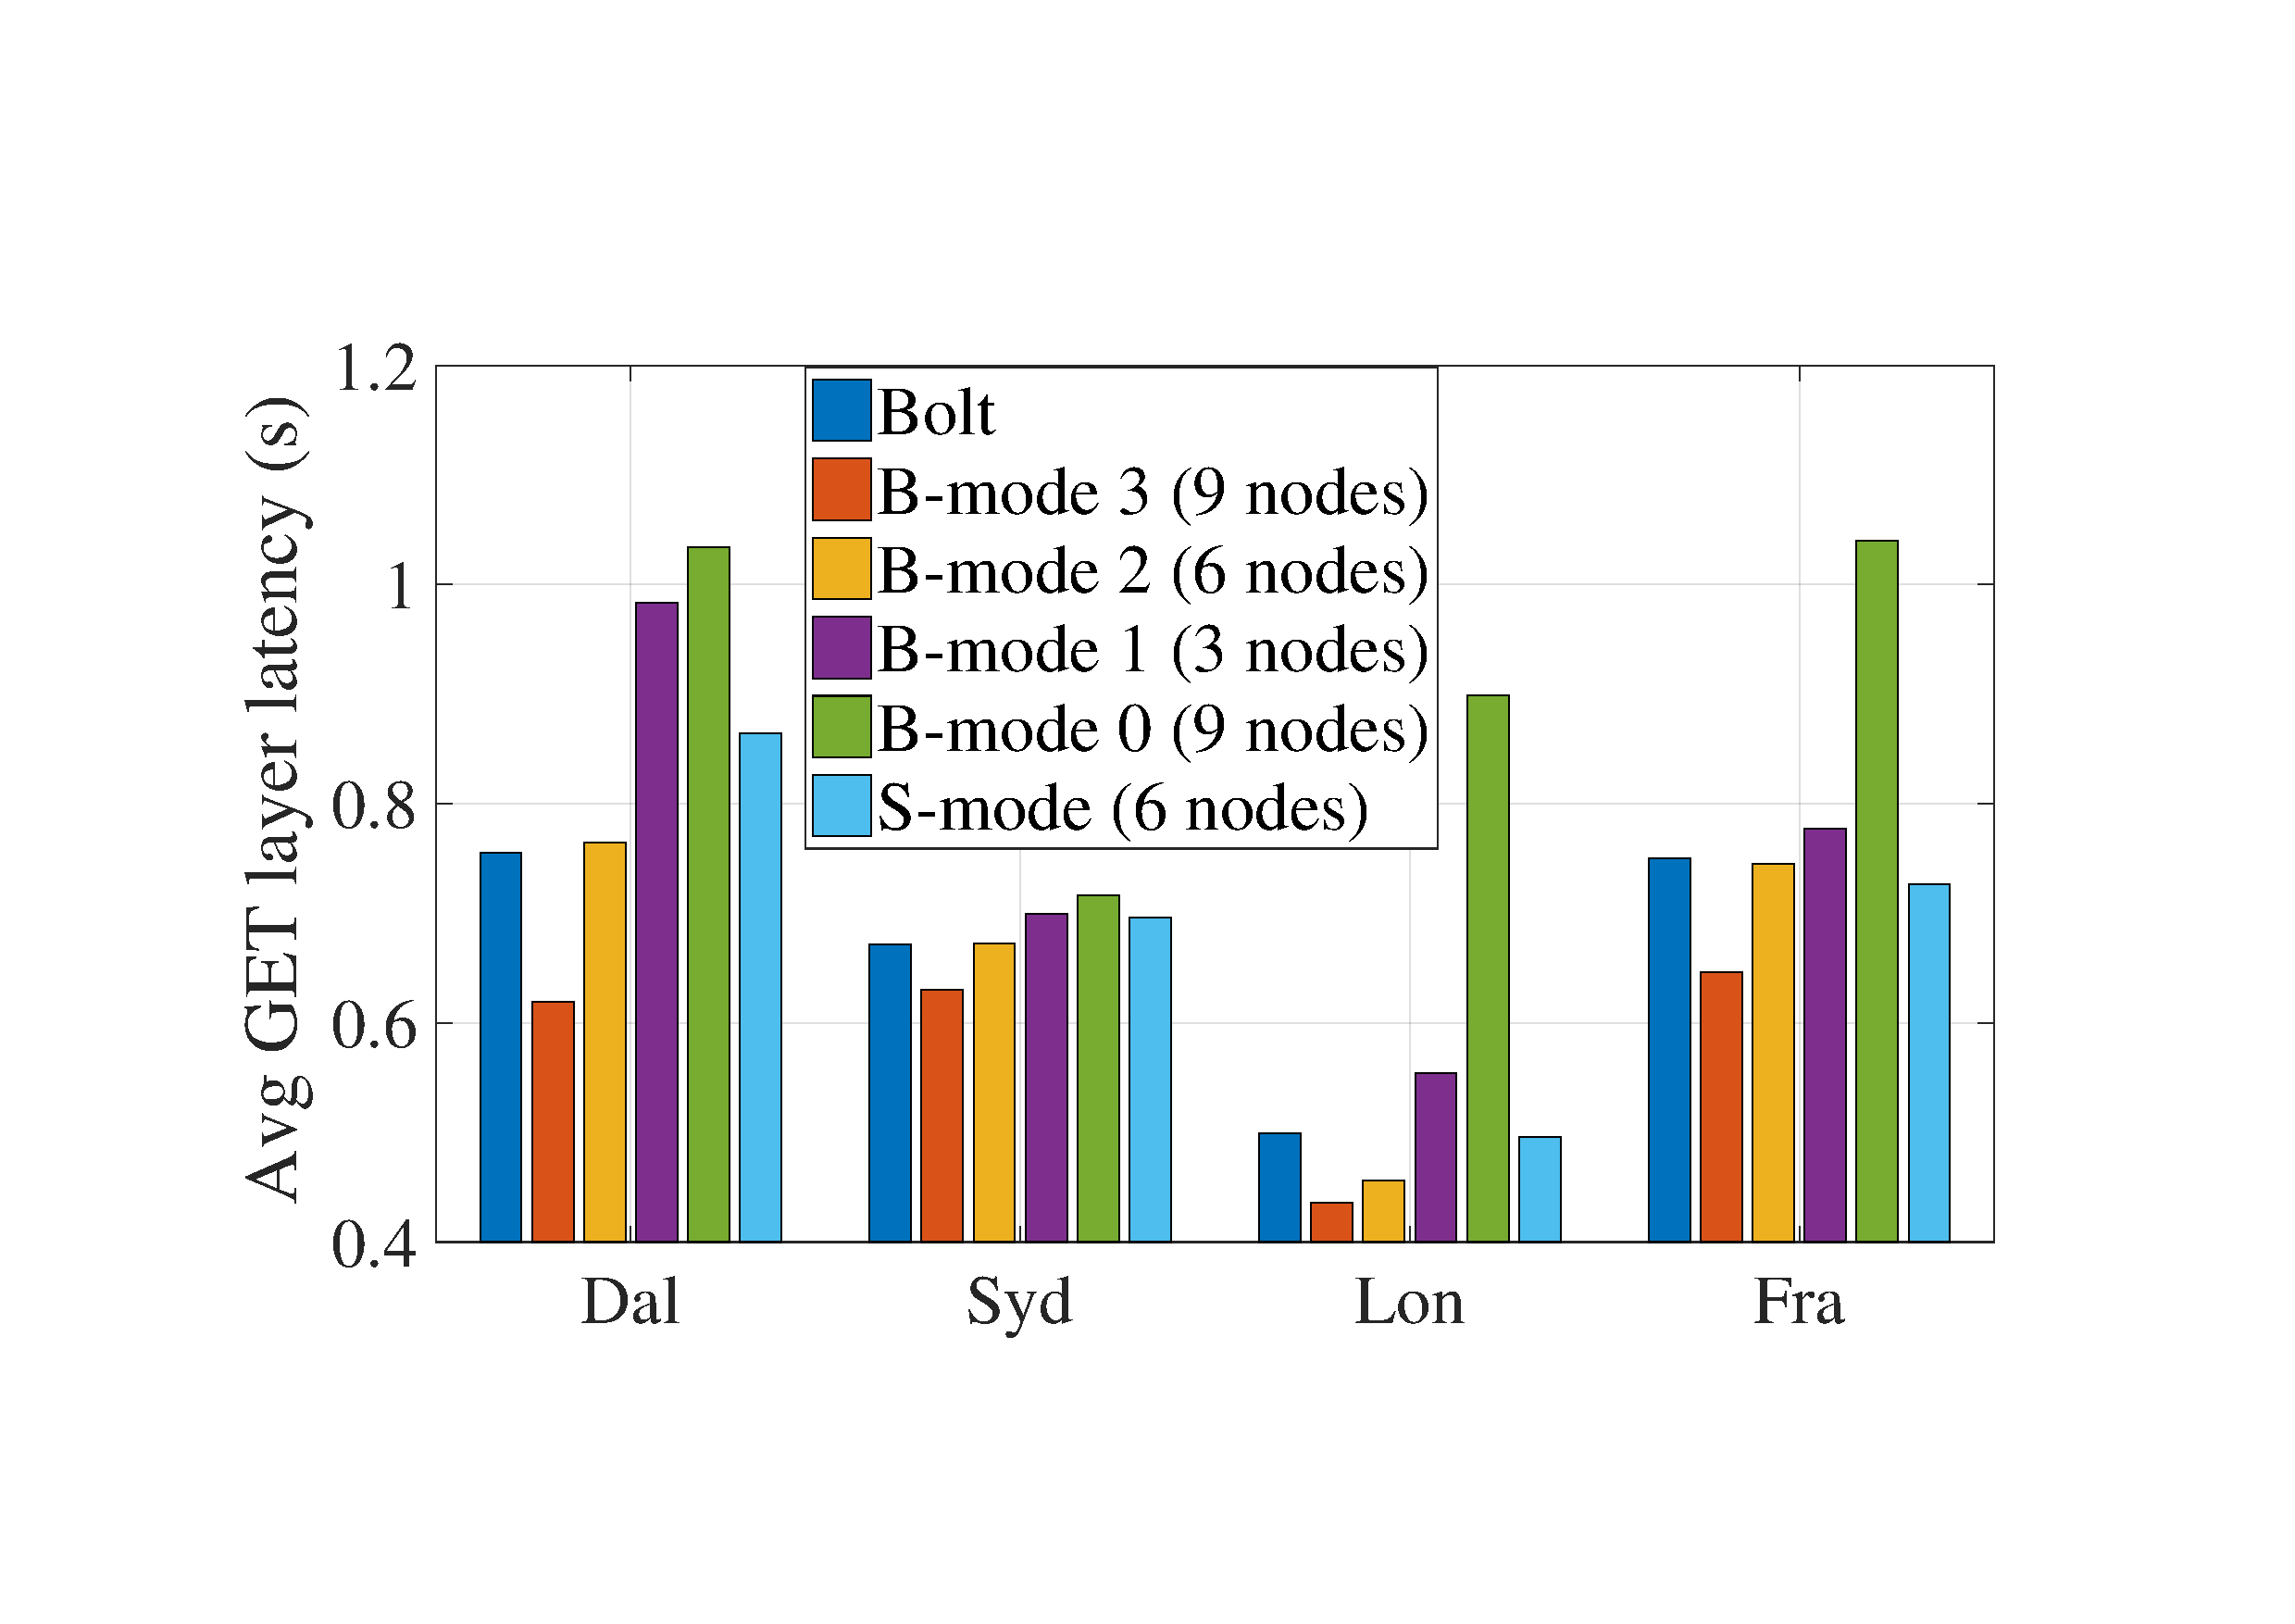
\includegraphics[width=0.9\textwidth]{graphs/total-traces.pdf}
%		\caption{Cache hit ratio.}% of LRU cache and preconstruct cache.}
%		\label{fig:eval-cachehitratios}
%	\end{minipage}%
%%	\begin{minipage}{0.3\textwidth}
%%	\centering
%%	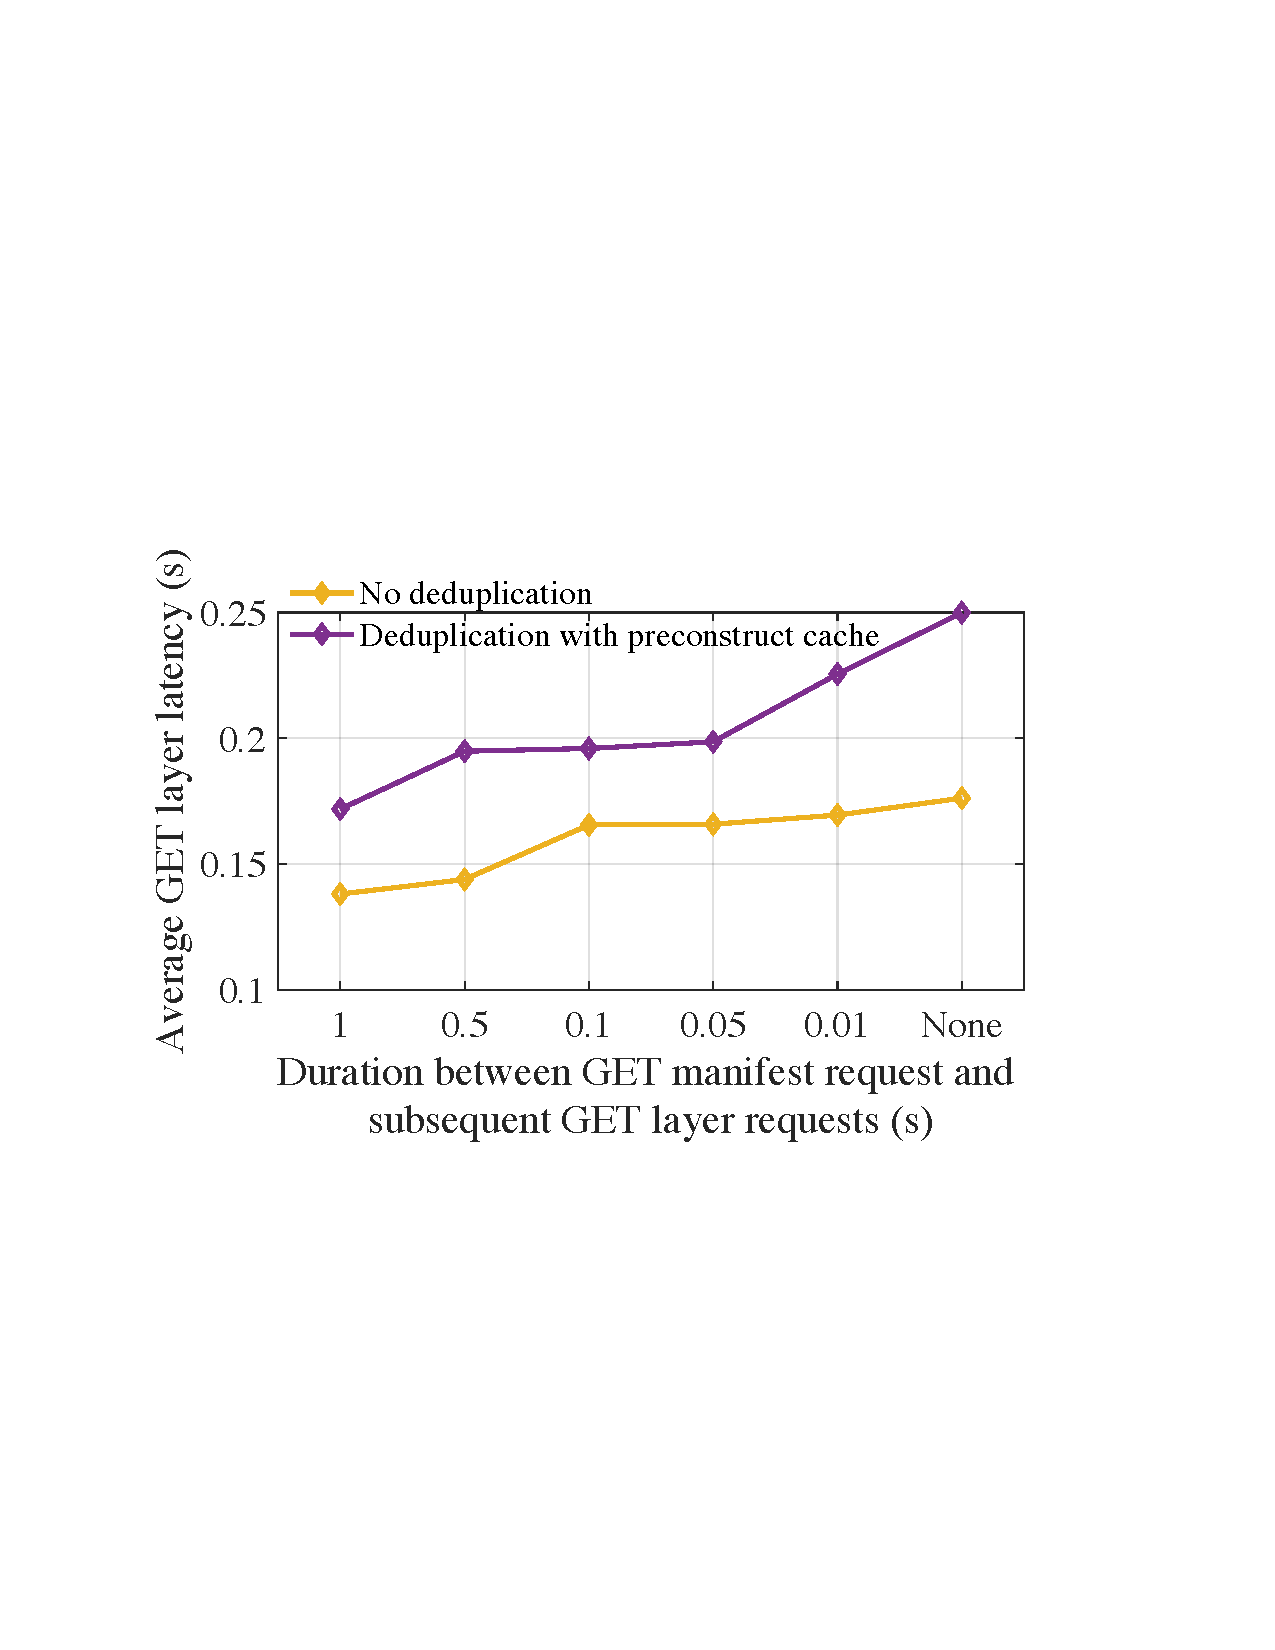
\includegraphics[width=0.9\textwidth]{graphs/durationML.pdf}
%%	\caption{The impact of durationML.}
%%	\label{fig:eval-durationML}
%%   \end{minipage}
%
%\end{figure}


\begin{figure}[t]
	\centering
	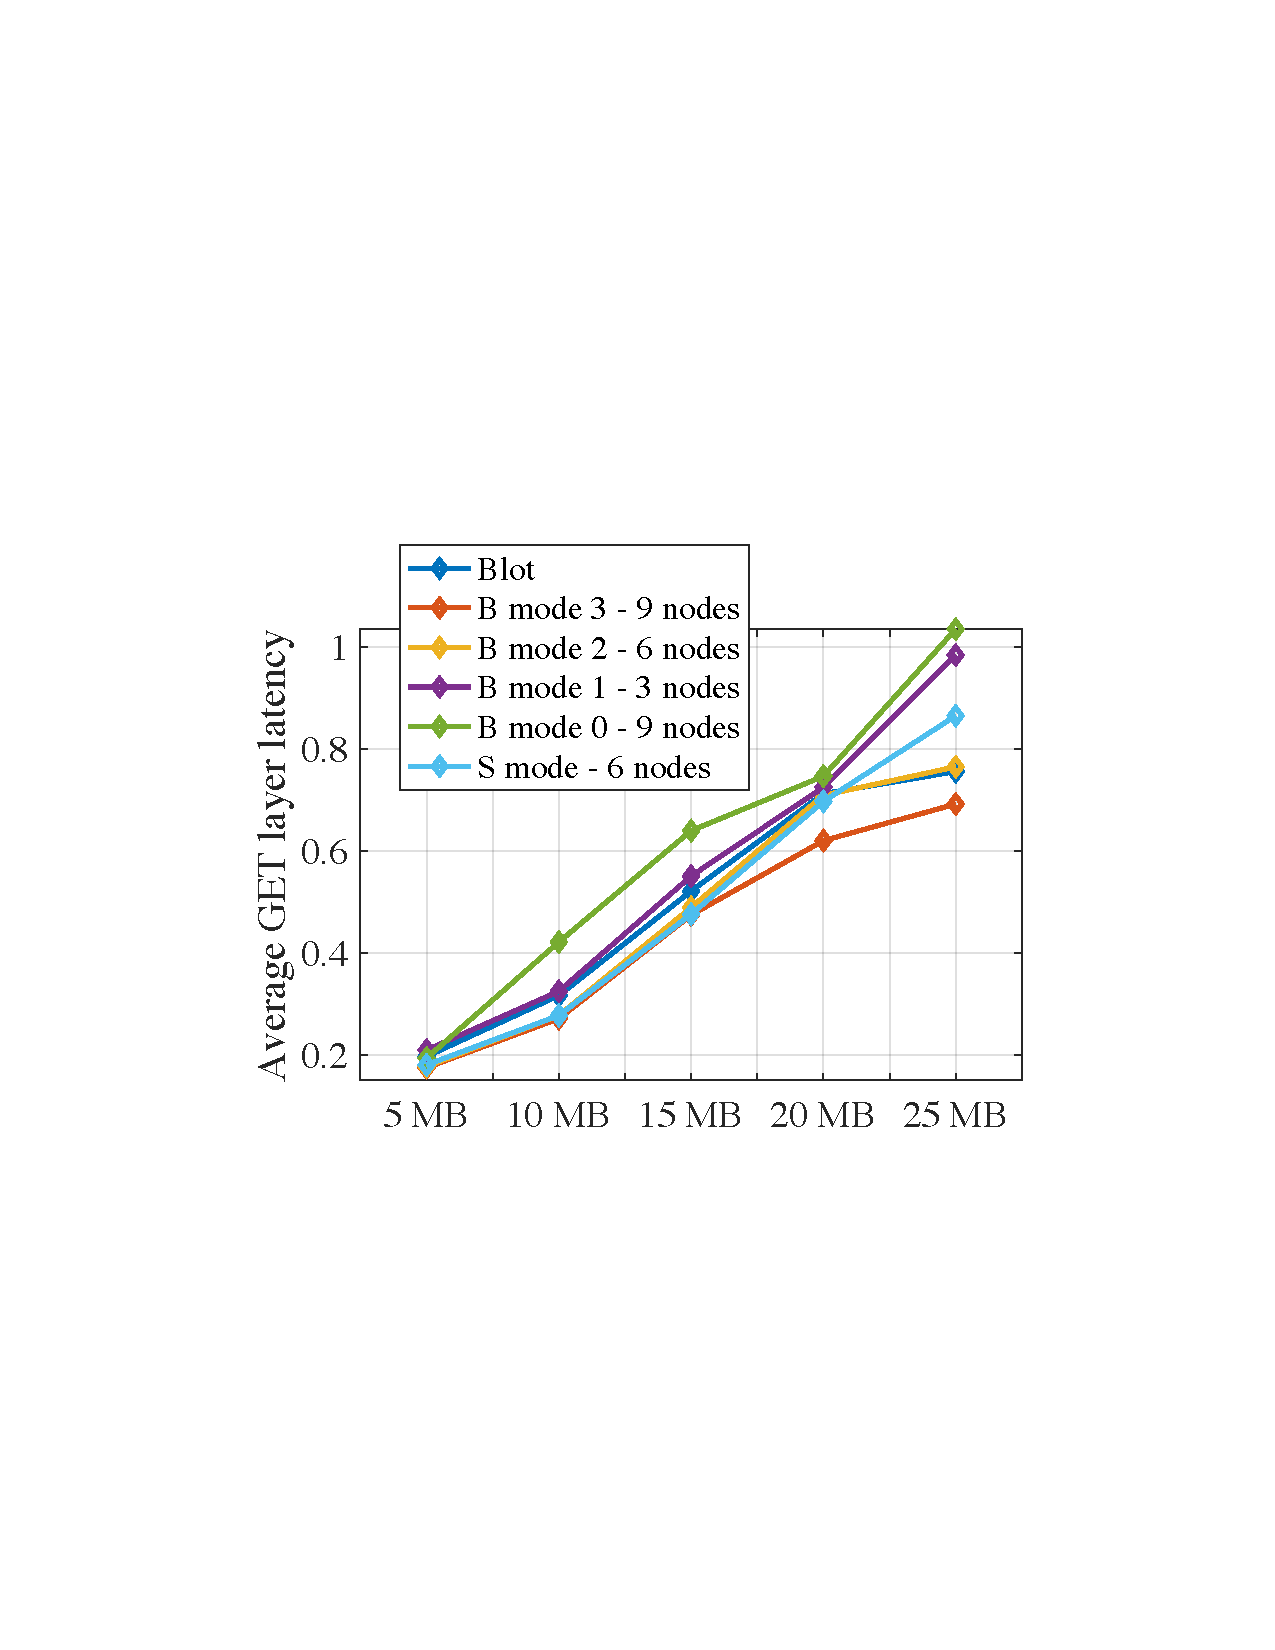
\includegraphics[width=0.4\textwidth]{graphs/dalprimary.pdf}
	\caption{Average \texttt{GET} layer latency.}
	%	\vspace{-3pt}
	\label{fig:eval-dalprimary}
	
\end{figure}

\begin{figure}[t]
	\centering
	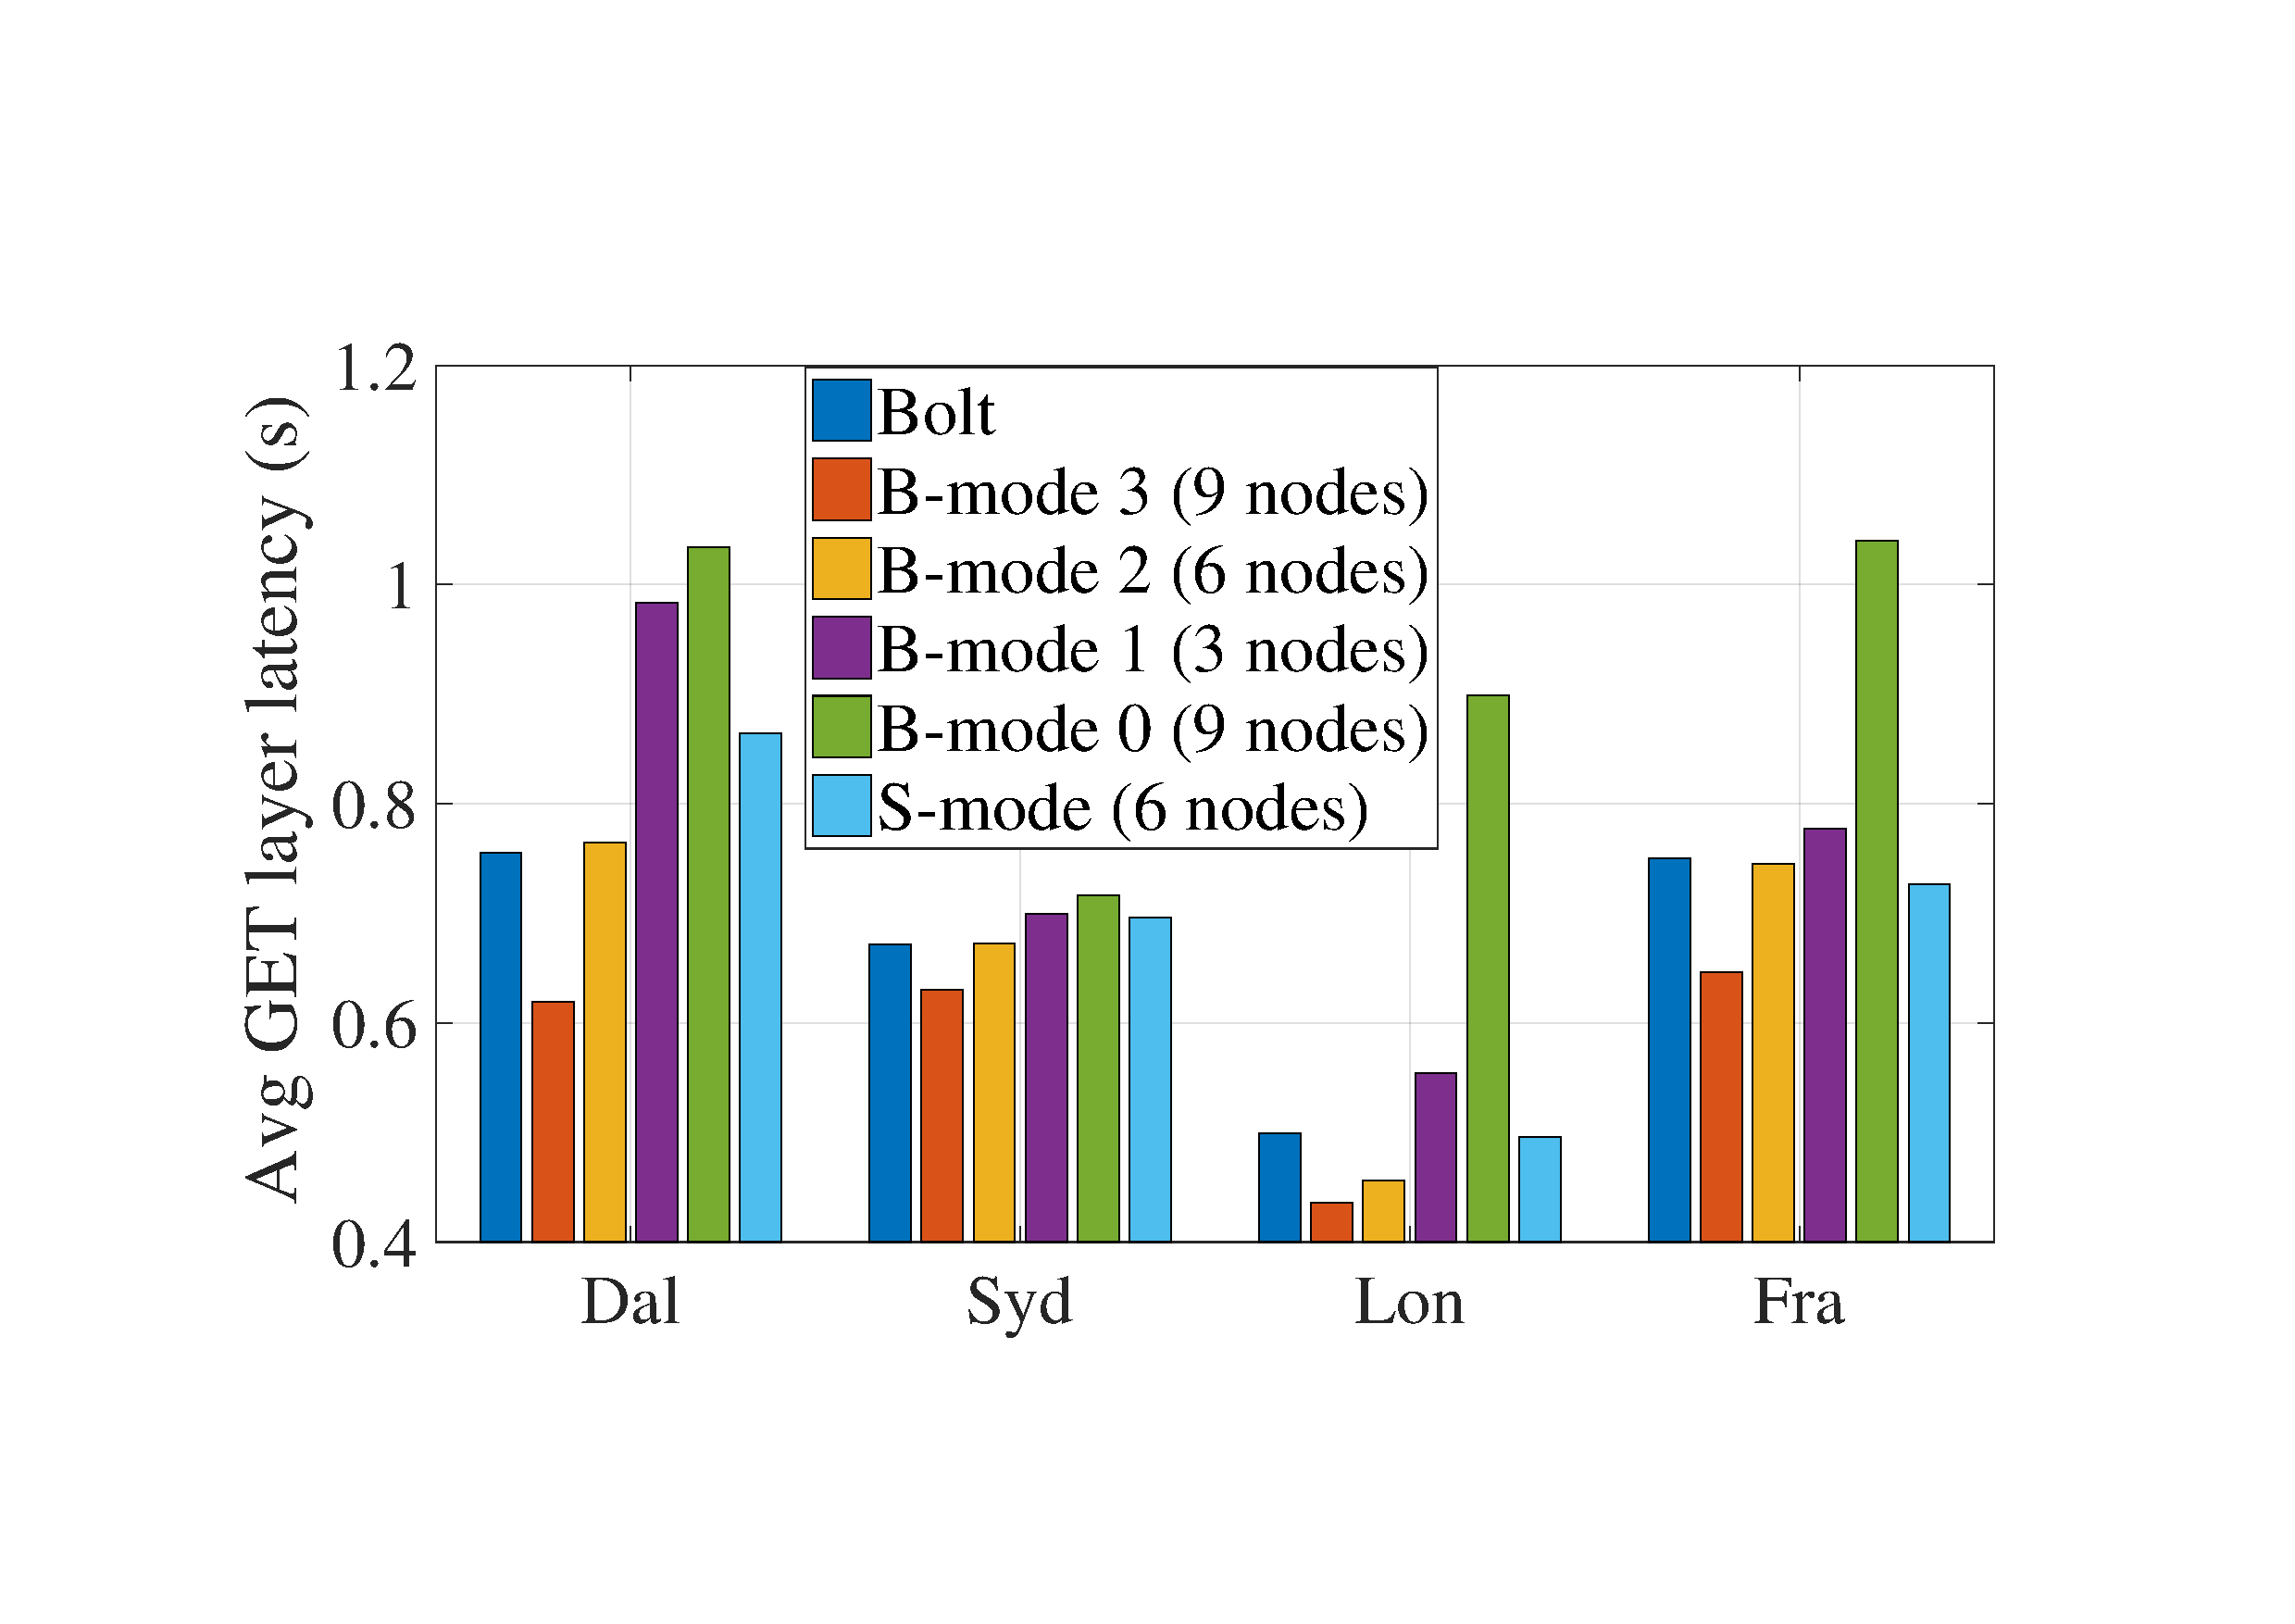
\includegraphics[width=0.4\textwidth]{graphs/total-traces.pdf}
	\caption{Average \texttt{GET} layer latency.} %\Subil{"Blot" in figure should be "BOLT".}}
	%	\vspace{-3pt}
	\label{fig:eval-total-traces}
	
\end{figure}

\subsection{Performance of primary cluster }
%\paragraph{}
In this experiment,
we test five modes of \sysname:
\textbf{B-mode 0},
\textbf{B-mode 1},
\textbf{B-mode 2},
\textbf{B-mode 3}, and
\textbf{S-mode}.
Note that B-mode 3 does not deduplicate layer replicas.
While B-mode 0 \emph{deduplicates} all layer replicas. 
%\sysname is evaluated by configuring different deduplication modes.
Therefore, B-mode 3 doesn't have P-servers while
B-mode 0 doesn't have P-servers.
For the remaining modes,
the number of P-servers and D-servers are set to 14 and 7 respectively.
%In addition, 
%we speedup trace replaying by using different speedup factors
%so that each trace can be finished within 30 minutes.
Before we replay each workload, we first warmup P-servers and D-servers with a certain amount of layers as shown in Table~\ref{tab:eval-overall}, which roughly takes 10 minutes.
Then, we use 32 clients spread between four client servers distributed on client cluster to replay traces to P-servers and D-servers.
We also evaluate the \emph{original registry} with 3-way replication on 21 servers. 

Figure~\ref{label} shows the average response time for \texttt{GET} layer, \texttt{PUT} layer, \texttt{GET} manifest, and \texttt{PUT} manifest requests for \sysname with different deduplication modes and original registry across different workloads.
Note that for \emph{B-mode 0}, the \texttt{GET} layer latency is the \emph{layer restoring latency}.

Overall, \texttt{PUT} requests have much higher average response time than \texttt{GET} requests.
For example, the average response time of 
\texttt{PUT} layer requests is almost twice higher than that of \texttt{GET} layer requests.
Note that registry servers use SSDs as secondary storage devices.
The difference in response time for \texttt{PUT} and \texttt{GET} requests are mainly caused by the different writes and reads throughput of SSDs. 

Comparing the \emph{original} with \emph{B-mode 3},
we see that \emph{B-mode 3} improves the overall performance by using a \emph{superfetch cache}.
\emph{B-mode 3}.
\emph{B-mode 3} reduces 5\% of average \texttt{GET} layer latency
and 32\% of average \texttt{PUT} layer latency compared with \emph{original} for workload \texttt{Dal}.
Next we compare \emph{B-mode 0} with \emph{original}.
Although \emph{B-mode 0} saves half of the storage space
by \emph{deduplicates} all layer replicas,
it slightly reduce \texttt{GET} layer latency by 6\%.
This is because of the high preconstruct cache hit ratio (detailed in Figure~\cite{xxx}), 
which reduces the layer restoring latency.

For the remaining basic modes: \emph{B-mode 2} and \emph{B-mode 1},
we see that \emph{B-mode 1} has a similar average response time to \emph{original}
although the primary cluster of \emph{B-mode 1} only has 14 nodes while 
\emph{original} contains 21 nodes.
This is because only a one-third of the %less data (1/3) 
data is \texttt{pushed} onto the primary cluster in \emph{B-mode 1}.
\texttt{Push} requests also affect the performance of \texttt{pull} requests
in terms of more network traffic and more writes to SSDs.
While \emph{B-mode 2} degrades \emph{GET} layer performance by 11\%.
This is because in \emph{B-mode 2},
more data (2/3) is \texttt{pushed} onto the 14-node primary cluster compared to \emph{B-mode 1},
which causes a lot of overhead.
\emph{S-mode} also has a similar \texttt{GET} layer performance with both \emph{original} and \emph{B-mode 1}.
This is because in \emph{S-mode}, only a few of the hot layers have 3 replicas while the remaining cold layers only have a single layer replica on the primary cluster. 

We find that
\emph{B-mode 1}, \emph{B-mode 2}, \emph{B-mode 0}, and \emph{S-mode}
 also improve the \texttt{PUT} layer performance by $\sim$ 30\% as \emph{B-mode 3}.
This is because
all 4 modes reduce the amount of \emph{pushed} layers to primary cluster results in
less network traffic and uses in-memory superfetch cache to reduce disk I/Os.
Similarly,
all modes improve \texttt{GET} and \texttt{PUT} manifest performance.
For example, \emph{B-mode 1} reduces \texttt{GET} and \texttt{PUT}
manifest latency by 17\% and 24\% respectively.

\paragraph{Cache hit ratio}

Figure~\ref{xxx},
shows superfetch cache hit ratio and preconstruct cache hit ratio.
Note that the superfetch cache is used by the primary cluster while the preconstruct cache is used by the deduplication cluster.
The superfetch cache hit ratio shown in Figure~\ref{xxx} is the average superfetch cache hit ratio across \emph{B-mode 3}, \emph{B-mode 2}, \emph{B-mode 1}, and \emph{S-mode} because they show the similar cache hit ratios.
Preconstruct cache hit ratio is measured in \emph{B-mode 0}.
Note that the big difference between a superfetch cache and a preconstruct cache is that the superfetch cache can prefetch layers \emph{on time} while the preconstruct cache cannot guarantee the preconstruction of layers \emph{on time} which makes a certain amount of \texttt{pull} layer requests \emph{wait} (detailed in~\ref{xxx}).
The cache size is set to 20\% of ingress data.

We see that the superfetch cache has a higher hit ratio than the preconstruct cache
because of the large amount of waiting layers on the preconstruct cache.
For example, for the preconstruct cache, 
the hit ratio is only 79\% excluding 20\% waiting layers requests for workload \texttt{Syd}.
while the hit ratio of the superfetch cache is 98\%.
The number of waiting layers vary across different workloads.
There are 4\% and 22\% of layer waits on the preconstruct cache for \texttt{Dal} and \texttt{Lon} respectively. 
Note that we speedup trace replaying
and the speedup factor for \texttt{Lon} is the biggest.
Trace replay speedup does not only decreases the idle time between \texttt{pull} image requests, it also reduces the duration between a \texttt{GET} manifest request and the subsequent \texttt{GET} layer requests.
Therefore, with the biggest speedup factor,
lots of layer preconstruction cannot be finished on time.
Moreover, for most of the workloads, the superfetch cache hit ratio is higher than 81\%. 
The \texttt{Dal} workload has the lowest hit ratio (0.77) because of the low prediction accuracy for \emph{users' repull behaviors} 
and the heaviness of the workload.

Figure~\ref{xxx} shows file cache hit ratio during layer restoring in \emph{B-mode 0}.
The file cache size is also set to 20\% of ingress data.
Overall, we see that file cache hit ratio is fair.
The hit ratio is lower than 60\% across all workloads, which means less files are shared among layers during a \emph{pull} image request.
It also means that the amount of shared/deduplicate files among layers is less when the accessed layer dataset is smaller.
Consequently, to get a higher deduplication ratio, deploying layer deduplication on a big layer dataset is a better choice, which aligns with~\cite{dedupanalysis}.




\paragraph{Client concurrency impact}
Figure~\ref{label} shows the average response time for different deduplication modes and for the original registry with 8 clients and 64 clients, respectively.

\paragraph{Primary cluster size  impact}
Figure~\ref{label} shows the average response time for different deduplication modes and for the original registry with a 7-node cluster and a 14-node cluster, respectively.
The number of concurrent clients are set to 32.
%\paragraph{Layer size impact}



%\subsubsection{Performance Vs. Space}

%\subsubsection{Performance }
%\section{Deduplication performance}
%\label{sec:Evaluation}
%
%%Our two-tier heterogeneous cache in the registry can improve the performance of the entire system
%%by hiding the long latency imposed by the backend dedup system.
%%Next, we present the preliminary evaluation of our user access history-based cache algorithm
%%and the space efficiency of file cache.
%
%\vspace{-6pt}
%\paragraph{Cache hit ratio.}
%
%We simulate our user-access-history-based cache and 
%replay the \texttt{dal} workload~\cite{dockerworkload} to measure the hit ratio. We set the cache size to be $20$\% of the data ingress for \texttt{dal}. We set $10$\% of the cache for buffering incoming \texttt{put} layer requests, and 
%the rest for caching prefetched layer slices from backend servers. 
%Note that in this evaluation, the cache only contains the layer buffer without the file cache.
%%as shown in Figure~\ref{fig:hitratio}.
%%Our algorithm exhibits an enhanced cache performance, with a high hit ratio
%%up to 0.96.
%Figure~\ref{fig:hitratio} shows the results. We observe a significant increase in the hit ratio, $74$\% to $95$\% as the duration threshold grows from $1$ to $10$ minutes. This is because prefetched layers are kept in the cache for more time.
%The hit ratio stablizes at $96$\% as the duration threshold increases from $15$ to $20$ minutes.
%%Therefore,
%%the highest hit ratio of our algorithm is around 0.96,
%%and there are 0.4 of layers that are miss because 
%%some users \emph{re-pull} the layers after they pull the same layers.
%The layers responsible for the $4$\% miss rate are the ones being
%\emph{re-pulled} by the same user.
%%We also see that 74\% of users can finish their \texttt{pull} layer request
%%within a minute and 
%%around 89\% of users can finished their \texttt{pull} layer request with less than 5 min. 
%%We also see that the response time to \texttt{pull} layer requests is within $1$ minute for 74\% of users, and it is less than $5$ minutes for 89\% of users.
%%Since we buffer layers upon a \texttt{push} layer request and prefetch layer {\em slices} from the backend servers, 
%%we compare the hits on prefetched layer {\em slices} and the hits on buffered layers.
%We see that, across different duration thresholds, 
%the hits upon buffering newly put requests (denoted as buffering hit ratio) is very low,
%confirming that it takes a long time for a recently \emph{pushed} layer to be pulled.
%We also observe a $22$\% average cache utilization. 
%That is because our algorithm is based on users demand 
%so it adapts to workload changes.
%%This trend is perfectly fit in our two-tier heterogeneous cache
%%and the evaluation results can guide us to carefully choose 
%%layer buffer size and file cache size.
%%
%%In terms of file count, it increases from \textbf{3.6$\times$} to \textbf{31.5$\times$} while
%%in terms of capacity, it increases from \textbf{1.9$\times$} to
%%\textbf{6.9$\times$} as the layer dataset grows from 1000 to 1.7 million layers.
%%%
%%This confirms the high potential for file-level deduplication in large-scale
%%Docker registry deployments.
%
%\vspace{-6pt}
%\paragraph{Space efficiency.}
%%As shown in Figure~\ref{xxx},
%%we compare the cache hit ratio of LRU, Prefetch~\cite{xxxx}, and our 
%%user-based cache replacement algorithm by replaying three IBM container registry workloads~\cite{dockerworkload}.
%%Our user-based cache exhibits an enhanced cache performance, with hit ratio improvements ranging from 
%%0.2 to 0.3 for all the three workloads compared to LRU.
%We analyze the space efficiency of the file cache compared to a cache that naively stores
%compressed layers.
%%for an increasing number of files stored in the file cache 
%%(see Figure~\ref{fig:dedup-ratio-growth}).
%%
%%Figure~\ref{fig:dedup-ratio-growth} shows the deduplication ratio growth over the layer dataset size.
%%
%In Figure~\ref{fig:cacheefficiency}, the x-axis values correspond to the sizes of $4$ random samples drawn from the whole dataset and the size of the dataset in terms of capacity and layer count.
%For a traditional cache, the compressed layer tarballs will be kept as is.
%While \sysname will store \emph{deduped} layers. 
%%unique files in the file cache.
%The y-axis shows how many more \emph{deduped} layers can fit in our file cache compared to naively storing compressed layer tarballs.
%For the first two samples of the dataset, with size less than $20$~GB, 
%there is no benefit to \emph{dedup} layers 
%because the deduplication ratio is very low.
%However, when the dataset size is $3$~TB, we can store $56\%$ more \emph{deduped} layers' unique files in file cache.
%The number of extra \emph{deduped} layers that can fit in the file cache increases almost linearly with the size of the layer dataset.
%%the bigger the dataset, the more deduped layers that can fit in the file cache.
%%The number of extra layers increases almost linearly with the layer dataset size.
%%In this case, there is a high potential for file cache when the cache size is big.
%This verifies the benefit of the file cache when the cache size is large, which should be carefully selected to realize significant space savings.


%In this experiment, we show how many more layers can be stored in the file cache 
%after decompression and file-level deduplication.
%Figure~\ref{xxxx} shows the growth of deduplication ratio with different dataset sizes.


%We evaluated \sysname's performance improvement over traditional 

%%While \sysname\ can effectively eliminate redundant files in the
%%Docker registry, it introduces overhead which can reduce the
%%registry's performance.
%%
%%The overheads can be classified in two categories: 1)~\emph{background
%%overhead} caused by the computation and I/O that is performed during layer
%%deduplication; and 2)~\emph{foreground overhead} from extra processing on the
%%critical path of a pull request.
%%\begin{figure}
	\centering
	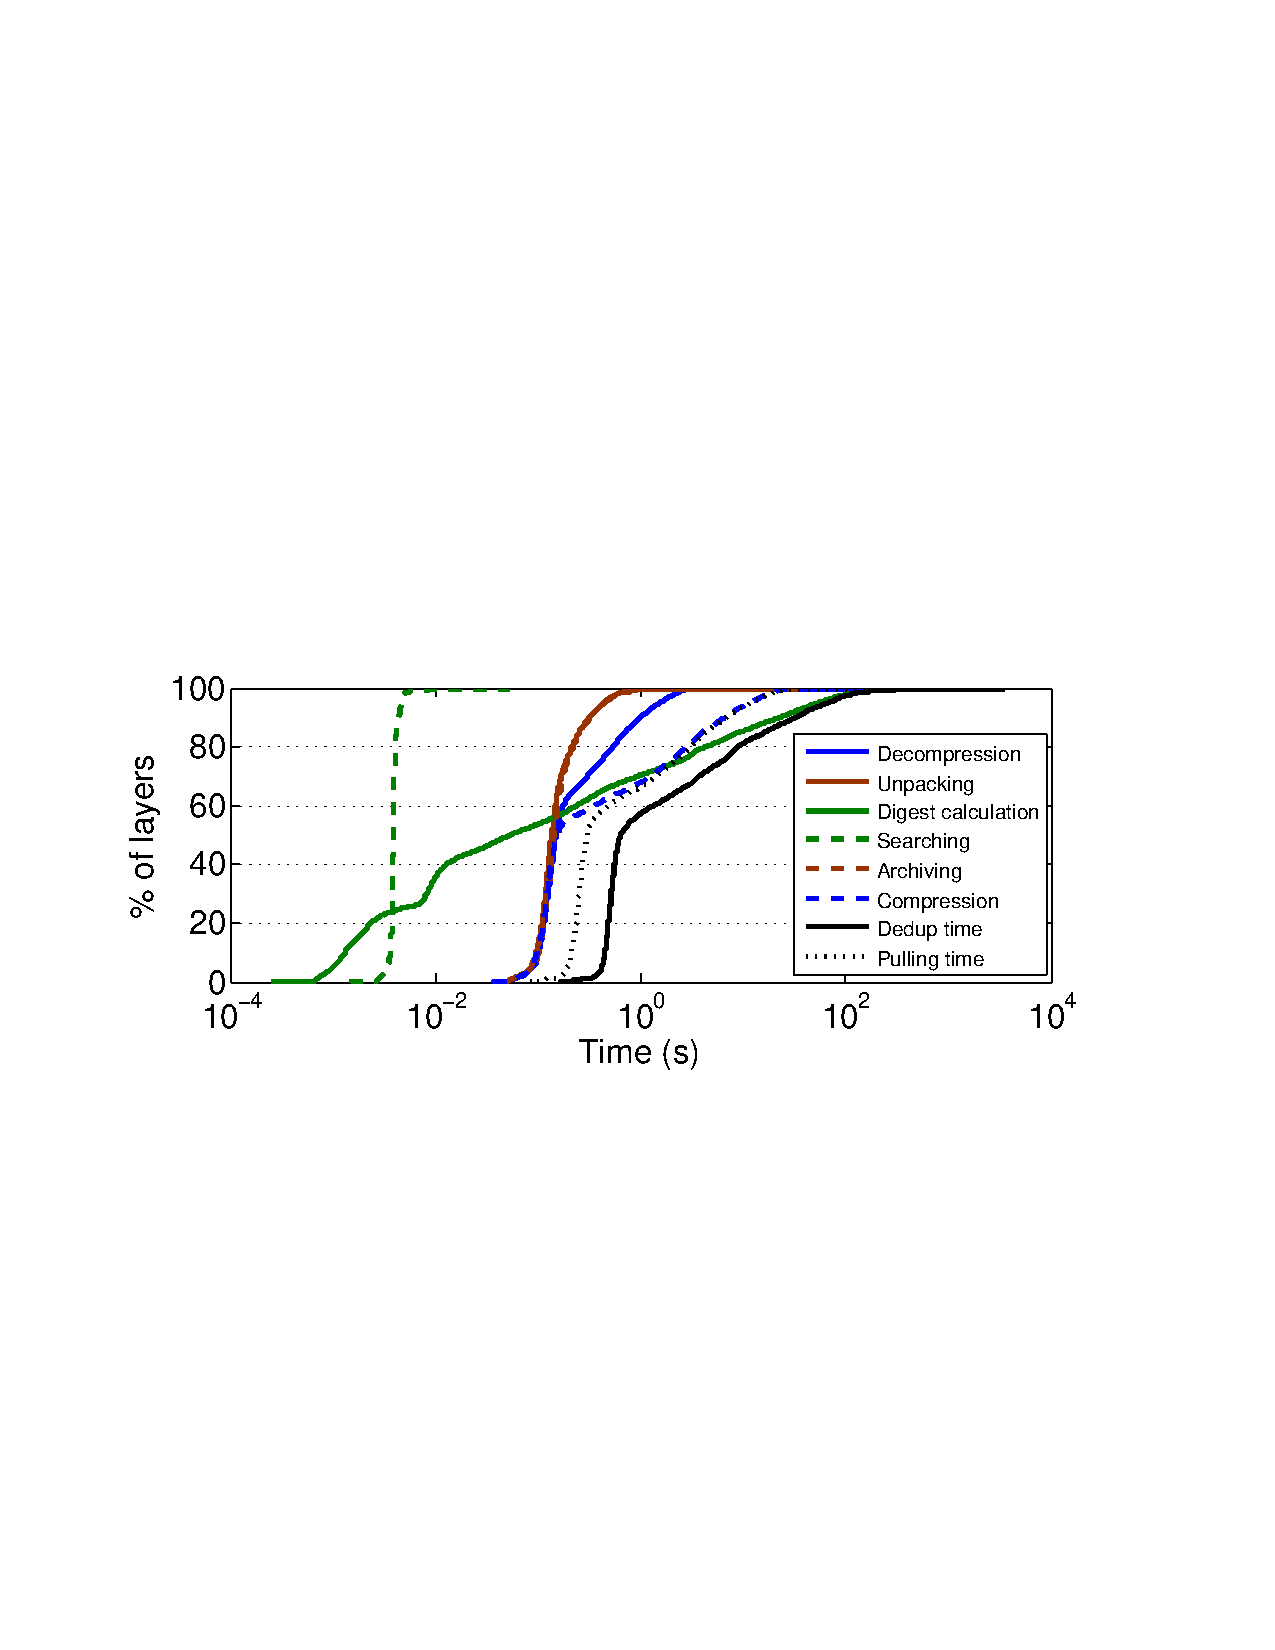
\includegraphics[width=0.5\textwidth]{graphs/res-time.pdf}
	\caption{Off-line file-level deduplication run time.}
	\label{fig:dedup-res}
\end{figure}

%
%
%%\paragraph{Hit ratios}
%%
%%\paragraph{Hit ratios with prefetching}
%%
%%%\subsection{} % what are the cost for a naive file-level deduplication
%%
%%\paragraph{Restoring performance breakdown}
%%
%%\paragraph{Simulation}
%%
%%To analyze the impact of file-level deduplication on the registry performance,
%%we conduct a preliminary simulation-based study of \sysname.
%%
%%Based on the simulation results, we estimated the overhead of \sysname\ on
%%\texttt{push} and \texttt{pull} layer request latencies.
%%
%%We then provide different suggestions on how the Docker registry can mitigate
%%the deduplication overhead.
%%
%%%%%%%%%%%%%%%%%%%%%%%%%%%%%%%%%%%%%%%%%%%%%%%%%%%%%%%%%%%%%%%%%%%%%%%%%%%%%
%%
%%
%Our simulation
%approximates several of \sysname's steps as described in Section~\ref{sec:design}.
%%
%First, a layer from our dataset is copied to a RAM disk. 
%%
%%
%%Note that there is no foreground pull or push requests since the simulation is \emph{off-line}.
%%
%The layer is then decompressed, unpacked, and the fingerprints of all files
%are computed using the MD5 hash function~\cite{MD5}.
%%
%The simulation searches the fingerprint index for duplicates,
%and, if the file has not been stored previously, it records the
%file's fingerprint in the index.
%%
%%To map a layer to its containing files, we create the layer recipe and add it
%%to a \emph{layer-to-file table}.
%%
%%The simulator then creates a file recipe.
%%
%%For each file in a layer, a layer digest
%%to its containing file content digest mapping record is also created 
%%
%%The \emph{layer-to-file table} also
%%records the file path within each layer associated with each file.
%%
%At this point our simulation does not include
%the latency of storing unique files.
%%
%To simulate the layer reconstruction during a \texttt{pull} request,
%we archive and compress the corresponding files.
%%
%%Only unique files are maintained in RAM
%%disk while the redundant copies are removed.
%%
%
%The simulator is implemented in 600 lines of Python code
%and our setup is a one-node Docker registry on a machine with 32~cores and 64\,GB of RAM.
%%
%To speed up the experiments and fit the required data in RAM
%we use 50\% of all layers and exclude the ones larger than 50\,MB.
%%
%We process 60 layers in parallel using 60 threads.
%%
%The entire simulation took 3.5 days to finish.
%%
%%The overall runtime is about 3.5 days.
%
%Figure~\ref{fig:dedup-res} shows the CDF for each sub-operation of
%\sysname.
%%
%Unpacking, Decompression, Digest Calculation, and Searching 
%are part of
%the deduplication process and together make up the Dedup time.
%%
%%\VT{@Nannan, in Figure ~\ref{fig:dedup-res} can you reorder the lines in the
%%legend so that the Searching goes after Digest calculation?}\NZ{addressed}
%%
%Searching, Archiving, and Compression
%simulate the processing for a \texttt{pull}
%request and form the Pulling time.
%%
%
%%\LR{What was the overall runtime for processing 0.9 million layers?}\NZ{addressed}
%%
%%\alicomment{How are we saving the location
%%of each file in the layer? It is not clear from the following sentences.}
%%\NZ{addressed}
%%
%%To improve searching performance, the
%%mapping table is stored in Hive database~\cite{xxx}. 
%%
%%\lrcomment{Why are we using Hive for this? It seems overkill to me, especially
%%for such small data. Even at scale, a KeyValue store would probably provide
%%better performance than clunky MapReduce-based DB.}
%%
%
%\paragraph{Push}
%
%\sysname\ does not directly impact the latency of \texttt{push} requests because
%deduplication is performed asynchronously.
%%ie the registry reliably stores a
%%copy of the layer as-is and then sends a response to the client.
%%
%The appropriate performance metric for \texttt{push} is the time it takes to deduplicate
%a single layer.
%%
%%Next, we look at the effects on \texttt{push} and \texttt{pull} latencies in
%%more detail.
%%
%%However, if there are intensive push requests while the registry is performing
%%deduplication, \sysname\ can still impact push latencies because it incurs
%%CPU, memory, and I/O overhead. %(similar to pull requests).
%%
%Looking at the breakdown of the deduplication time in
%Figure~\ref{fig:dedup-res}, we make several observations.
%
%First, the searching time is the smallest among all operations with 90\% of the
%searches completing in less than 4\,ms and a median of 3.9\,ms.
%%
%%The mapping table maintains 0.98 million layer-to-file digest mapping records. 
%%
%%\LR{Remove the following sentence? 1.7 million records is actually quite small
%%so even a single-node DB with one index is enough.}\NZ{addressed} Consider
%%that more than 1.7 million layers are stored in Docker hub and the number is
%%still increasing, it's better to choose a fast distributed database to provide
%%high searching performance and scalability.
%%
%Second, the calculation of digests spans a wide range from 5\,$\mu$s to almost
%125\,s.
%%
%%This is because the time mainly depends on the layer size, \ie the fewer and
%%smaller files a layer contains, the faster it is to compute all digests for
%%the layer.
%%
%%Typically, smaller layers contain a smaller number of smaller files, which
%%takes much less time to calculate their digests.
%%
%%While if the layer is bigger, the digest calculation overhead will be higher. 
%%
%90\% of digest calculation times are less than 27\,s while 50\% are
%less than 0.05\,s.
%%
%The diversity in the timing is caused by a high variety of layer sizes both in
%terms of storage space and file counts.
%%
%%Thus, we suggest that multiple-threading is needed to calculate the files'
%%digests simultaneously; 
%%
%%Fast CPUs as well as more powerful computing nodes are required to speed up
%%digest calculation.
%%
%Third, the run time for decompression and unpacking follows an identical
%distribution for around 60\% of the layers and is less than 150\,ms.
%%
%%Around 60\% of decompression and unpacking time are less than 0.15\,s. 
%%
%However, after that, the times diverge and decompression times increase faster
%compared to unpacking times.
%%
%%\VT{do we have some theory why?}
%%\NZ{decompressing the layers with bigger uncompressed size takes longer time.}
%%
%90\% of decompressions take less than 950\,ms while 90\% of packing time is less
%than 350ms.
%
%%Overall, we see that file digest calculation contributes a lot to the
%%overall deduplication latency especially when the layer size is big.  Moreover,
%%we see that the deduplication latency increases as the layer size grows.
%%
%Overall, we see that 90\% of file-level deduplication time is less than 35\,s
%per layer, while the average processing time for a single layer is 13.5\,s.
%%
%This means that our single-node deployment can process about 4.4\,layers/s on average
%(using 60 threads).
%%
%In the future we will work on further improving \sysname's deduplication throughput.
%%
%%In a large-scale registry deployment, this throughput can be improved
%%as more node are available to perform deduplication.
%%
%
%\paragraph{Pull} 
%
%From Figure~\ref{fig:dedup-res}
%we can see that 55\% of the layers have close compression and archiving
%times ranging from from 40\,ms to 150\,ms and both operations contribute equally
%to pulling latency.
%%
%%60\% of compression and archiving time are less than 0.15 s.
%%
%%While compression has the highest run time 80\% of compression time is less than 2.82~s. 
%%
%%\LR{Again, better to show the 90th percentile.}
%%\NZ{90\% of the compression time is less than 8\,s.}
%After that, the times diverge and compression times increase faster with an
%90\textsuperscript{th} percentile of 8\,s.
%%
%This is because compression times increase for larger layers and follow the distribution
%of layer sizes (see Figure~\ref{fig:layer-size-cdf}).
%%
%%80\textsuperscript{th} percentile of 2.82\,s.
%%
%Compression time makes up the major portion of the pull latency and is a
%bottleneck.
%%
%Overall, the average pull time is 2.3\,s.
%
%%
%%We see that archiving time and compression contributes equally to pulling
%%latency when their run time are lower than 0.15 s while compression time almost
%%equals to pulling latency when the compression time is greater than 0.15 s. 

%\subsection{Restoring performance breakdown}

We breakdown \sysname's layer restoring performance in \emph{B-mode 0}
with 32 clients on 21-node cluster as shown in Figure~\ref{xxx}.% by using different number of D-servers.
%Before we replay traces on the D-server cluster, 
%We first warmup D-servers with a certain amount of layers for each workload as shown in Table~\ref{tab:eval-overall}.
%After that,
%and save each unique file with three file replicas.
%After all warmup layers are deduplicated and discarded,
%we use 32 clients to replay the workloads on D-server cluster 
%and measure the \texttt{GET layer} performance as layer restoring performance.
%We use 32 clients.
%Figure~\ref{xxx} shows layer restoring performance changes with different number of D-servers.
%the layer restoring performance compared with the layer \texttt{pulling} performance of original registry

%\paragraph{Cluster scale impact}

%\paragraph{Deduplication cluster size impact}

%\paragraph{Client concurrency impact}

%\paragraph{Cache impact}

%\paragraph{Preconstruct cache hit ratio}

%\paragraph{Breakdown performance}

%\paragraph{Client concurrency impact}

\paragraph{Waiting layer latency}

\paragraph{Layer size impact}


%\subsection{Deduplication performance}

We measure \sysname's deduplication performance in \emph{B-mode 0}
with 32 clients on a 21-node cluster.
%We use 32 clients to warmup D-servers with a certain amount of 
%layers as shown in Table~\ref{tab:eval-overall},
%After receiving the layers, D-server cluster performs layer deduplication and 
%save each unique file with three file replicas. 
%and measure the layer deduplication performance.

%\paragraph{Deduplication performance}

\paragraph{Breakdown performance}



